% Two sided means the left and right margins are different sizes and they alternate every page. 
% If your document is printed to be book or spiral bound this allows for a thick spine to not 
% eat into the space for your page content. 
\documentclass[11pt, a4paper, twoside, openright]{custard}

% All imports, packages, and configuration in here. 
% Your document should be about content so we abstract away the styling rules and tools we are using. 
%% Here you can specify new commands and environments that you intend
%% to use. Using commands can make your document easier to write, read
%% and be more consistent.

\usepackage[linesnumbered,ruled]{algorithm2e}
\DeclareMathOperator*{\argmin}{arg\,min}

\usepackage{appendix}
\usepackage{textcomp}
\usepackage{setspace}
%\usepackage[document]{ragged2e}
\usepackage{verbatim}
\usepackage{multirow}
\usepackage{multicol}
\usepackage{booktabs}
\usepackage{enumitem}
\sloppy
\usepackage{graphicx}
\usepackage{threeparttable}
\usepackage{epsfig}
\usepackage{epstopdf}
\usepackage{float}
\usepackage{enumitem}
\usepackage{cite}
\usepackage[export]{adjustbox}
\usepackage{algorithmic}
\usepackage[nohyperlinks,printonlyused]{acronym}
\usepackage{amsmath}
\usepackage{amsfonts}
\usepackage{array}
\usepackage{tabularx}
\usepackage{longtable}
\usepackage{times}
\usepackage{amssymb}
\usepackage{hhline}
\usepackage{color}
\usepackage{soul}
\usepackage{colortbl}
\definecolor{Gray}{gray}{0.85}
\usepackage{rotating}
\usepackage{fix2col}
\usepackage{pdflscape}
\usepackage{pdfpages}
\usepackage{stmaryrd}
\usepackage[export]{adjustbox}
\usepackage{bbm}
\usepackage{relsize}
\usepackage{xfrac}
\usepackage{bibentry}

%\usepackage{refcheck}

%watermarking
\usepackage[english]{babel}
\usepackage{tikz}

%% Uncomment the following line for hyper links - not recommended for printing
\usepackage[colorlinks, linkcolor=, anchorcolor=, citecolor=, filecolor=, menucolor=, runcolor=, urlcolor=]{hyperref}

\setcounter{tocdepth}{1}
%\setcounter{minitocdepth}{3} 
\linespread{1.31}

\newcommand\litem[1]{\item{\bfseries #1:\enspace}}

\interdisplaylinepenalty=2500

\newcolumntype{L}[1]{>{\raggedright\let\newline\\\arraybackslash\hspace{0pt}}m{#1}}
\newcolumntype{C}[1]{>{\centering\let\newline\\\arraybackslash\hspace{0pt}}m{#1}}
\newcolumntype{R}[1]{>{\raggedleft\let\newline\\\arraybackslash\hspace{0pt}}m{#1}}

\renewcommand{\thefootnote}{\fnsymbol{footnote}}
\setlength{\LTpre}{-10pt}\setlength{\LTpost}{-30pt}%
\newcommand{\oiint}{\begin{picture}(0,0)(-10,-2)\put(0,0){\oval(12,8)}\end{picture}\iint}
\renewcommand{\mathbf }{\boldsymbol}

\def \eg{e.g.\ } % Allows you to write \eg in LaTeX instead of typing e.g. so that every single one will be formatted the same.
\def \Eg{E.g.\ } % Define some other common variants. If you later want to change one of these definitions, 
\def \ie{i.e.\ } % it will update all the usages throughout the document.
\def \Dr{Dr.\ }
\def \vs{vs. }
\def \etal{\emph{et al.\ }} 
\def \sota{state-of-the-art }
\def \handcrafted{hand-crafted }

\usepackage{listings,lstautogobble}
\usepackage{sourcecodepro}
\pdfmapfile{=SourceCodePro.map}
\lstset{
	xleftmargin=0.5cm,frame=tlbr,framesep=4pt,framerule=0.5pt,
	language=,
	upquote=true,
	columns=fixed,
	tabsize=2,
	extendedchars=true,
	breaklines=true,
	numbers=left,
	numbersep=10pt,
	basicstyle=\ttfamily\scriptsize,
	numberstyle=\tiny,
	stringstyle=\ttfamily,
	captionpos=b,
	showstringspaces=false,
	autogobble=true
}

\usepackage[font=small,skip=10pt]{caption} %,format=hang
%\usepackage[labelformat=simple]{subcaption}
\usepackage[labelformat=simple]{subfig}
%\captionsetup[figure]{format=hang}
%\captionsetup[lstlisting]{format=hang}
\renewcommand{\thesubfigure}{\Alph{subfigure}.}

\renewcommand{\thefootnote}{\arabic{footnote}}

% Use IEEEtran citation style. 
\bibliographystyle{IEEEtran} 

\def\samplefont#1{%
    % set font style and save name
    #1\edef\savedname{\fontname\font}%
    % print small sample
    {\leavevmode\tt\hbox to 1in{\savedname:\hss}}%
    abcxyz ABCXYZ 123\par
}

\begin{document}
	
% The custom data for Swansea University and your degree name.
% The \protect\\ command forces a new line in the title which might be otherwise overriden by the template
	\title{GAN-EOT - Generative network for 3D black-box adversarial attacks}
	\author{Alexandru Dascălu\protect\\{\normalsize 965337}}
	\awardinginst{Swansea University}
	
	\degree{Master of Science}
	
% Institution details and logo
	\department{Department of Computer Science}
	\university{Swansea University}
	\unilogo{graphics/swansea.png}
	
% Hard code the date or allow the LaTeX compiler to fill it in whenever you recompile the document.
	\date{\today}
	
% Build the title and declaration pages, and pad the document so the text starts on a right hand book page.
% Page numbering is in roman numerals until the first page of an actual chapter which resets numbers 
% starting from 1 at that point. 
	\frontmatter%
	\maketitle
	\declaration
	\cleardoublepage
	
% Most books and theses have a brief foreword or dedication. 
	\begin{vplace}[0.7]
		\begin{large}
			\begin{center}
				\textit{I would like to dedicate this work to my family, for raising me and supporting me to be where I am now.}
			\end{center}
		\end{large}
	\end{vplace}

% Abstract comes before the contents page.	
	\begin{abstract}
		\vspace{-2em}
		\setcounter{page}{1}
		
		In your abstract you should aim to summarize the core contributions of your work in the context of the problem domain. Start by outlining the domain and the problems posed within it. Discuss how the methods you focus on approach the relevant problems. You should end your abstract by concretely stating the tangible outputs and deliverables you have created in order to complete your work on this document, and whether those outputs represent and improvement or alternative approach to existing methods. 
		
		Your abstract should be a couple or so paragraphs long, and roughly approximate the order and flow you then use for structuring the main document. If a viewer has read your abstract then they should already understand at a high level what it is you have created and delivered, and whether it is better than or comparable to existing methods. If your project is driven by a research hypothesis then the reader should know what that is at a high level from this section. Reading on, little should surprise the viewer.
		
		For paper submission of your thesis you should physically sign your name on each of the above declaration statements and date them in black ink. For digital submissions you should sign and date them digitally using a touch or stylus input if available. There are pieces of software that allow you to write directly on PDF documents, or alternatively you can bring a signature into your document as a figure with a transparent or white background. If you do not have a stylus input / tablet like device you should ask your supervisor, as many in the department do their grading / work on digital tablets.
	\end{abstract}
	
% A long form dedication. 
	\begin{Acknowledgements}
		First of all, I would like to express my deep gratitude to my mother for all the emotional support and encouragement that she has given me over the past academic year and for being there when I needed her.
		
		Furthermore, I would like to thank Dr. James Deng for being a great supervisor and for guiding me towards realistic project goals.
		
		Finally, I am thankful to my former coursemate Avi Varma for his support and suggestions and want to thank him for sharing with me things he learnt when doing his project a year ago.
	\end{Acknowledgements}
	
% Build the table of contents page.
    \setcounter{tocdepth}{2}
	\tableofcontents
	 
% Optionally you can make a bank of known acronyms in acronyms.tex that you can call on throughout your document.
	%\input{acronyms} 
	
% For long documents like a Doctoral thesis you should include a list of tables and figures throughout 
% your document. This is uses a shortened version of each table and figures caption and enumerates all 
% of them with their table or figure number. This is automatic, you do not need to modfy it if you do use it.
	\setlength{\columnsep}{10pt}
\newpage
\listoftables
\mtcaddchapter 
\newpage
\listoffigures
\mtcaddchapter  
	
% Reset numeric page numbering from page 1
	\mainmatter%

% Insert the code for each of your chapters
	\chapter{Introduction}
	\label{chap:intro}

Over the past 10 years, deep neural networks have advanced tremendously, and have been used for safety and security-critical tasks, such as face recognition \cite{face_recognition}, self-driving cars \cite{self_driving_cars} and malware detection \cite{malware_detection}. However, neural networks are vulnerable to a variety of attacks which enable malicious agents to manipulate their outputs \cite{deep_leakage, trojan_attacks, poisoning_attacks, szegedy2014intriguing}. Adversarial attacks are one such class of attacks. First discovered in 2014 by Szegedy \textit{et al.} \cite{szegedy2014intriguing}, they involve crafting special perturbations that are added to the original input to make the victim model predict a wrong label. Moreover, these perturbations are often imperceptible to humans \cite{szegedy2014intriguing}, and can fool a model into outputting specific wrong labels which are very different to the ground truth.

Since then, researchers have proven that attacks in the physical world \cite{evtimov_road_signs} and in cyberspace \cite{papernot_cyberspace_attack} are possible. For example, Eykholt \textit{et al.} \cite{evtimov_road_signs} successfully performed an adversarial attack that fooled a road sign recognition model in real life. Athalye \textit{et al.} \cite{athalye} created physical 3D objects that consistently fool neural networs for object recognition, regardless of the camera angle. This was in contrast to traditional attacks that create 2D adversarial images, as those are much less effective when printed and physically held in front of a camera \cite{lu_physical_experiments}. Consequently, the existence of adversarial examples undermines the safety of neural networks, and thus their applicability in safety or security critical systems.

One disadvantage of the physical world attacks created in \cite{athalye} and \cite{evtimov_road_signs} is that they are \textbf{white-box} attacks, they require access to the victim model. This is because they rely on gradient-descent optimisation and thus need to differentiate through the victim model. Another line of research looked at \textbf{black-box} attacks, which do not have this requirement \cite{akhtar}, and are thus more practical for the attackers. However, the black-box attacks in the literature only create 2D adversarial examples in the lab setting and are less effective in a physical scenario.

An adversarial attack that is both black-box and applicable to the physical domain would be especially practical for attackers. Therefore, my project will try to combine the framework used in Athalye \textit{et al.} \cite{athalye} and the generative model presented in \cite{zheng_black_box_GAN} to create a black-box adversarial attack which produces 3D rendered objects that can consistently fool object classifier neural networks. The findings may be useful for further understanding of adversarial attacks and for creating better defence methods.

The rest of this chapter is organised as follows: section \ref{sec:motivation} further details the motivation behind the project, section \ref{sec:scope_limitations} explains the scope and limitations, section \ref{sec:aims_objectives} lays out the aims and objectives and section \ref{sec:intro_contribs} explains the contributions of this work. The rest of the thesis is organised in the following way: chapter \ref{chap:background} provides the literature background, chapter \ref{chap:methodology} describes the research methodology and proposed architecture, chapter \ref{chap:results} contains the experiment design and results along with a discussion of said results, and chapter \ref{chap:conclusion} summarises the contributions of this project and mentions future work to build upon this thesis.

\section{Motivation}
    \label{sec:motivation}
	
Adversarial attacks are often highly effective at fooling a victim model \cite{akhtar, silva_survey, dong2020benchmarking, robustart, fgsm}. Hendrik Metzen \textit{et al.} \cite{Metzen_2017_ICCV} attacked an image segmentation neural network for use in a self-driving car. They managed to make the victim model not perceive pedestrians, as 84.5\% of pixels making up pedestrians were misclassified. If an attacker were to implement it in real life, the self-driving car could have run over pedestrians, because it would not see them, as figure \ref{fig:adversarial_segmentation} on page \pageref{fig:adversarial_segmentation} shows. Therefore, adversarial examples are a clear threat to neural networks used in safety-critical systems.

\begin{figure}[ht]
    \centering
    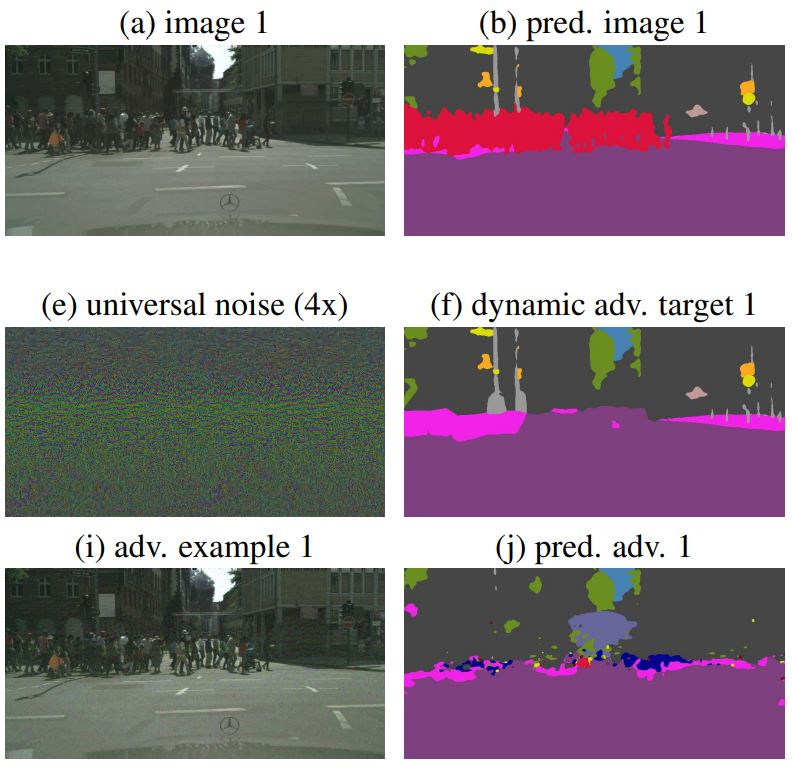
\includegraphics[width=0.75\textwidth]{graphics/adversarial_segmentation.JPG}
    \caption[Example of an adversarial example against neural network used in self-driving car.]{Example of an adversarial attack which removes pedestrians from the perception of a scene by a neural network. The top row contains the original image and the correct image segmentation. The middle row shows the adversarial noise and the target segmentation, which has the pedestrians removed from the scene. The last row shows the adversarial example and the predicted segmentation. Taken from \cite{Metzen_2017_ICCV}.}
    \label{fig:adversarial_segmentation}
\end{figure}

Most attacks, including the one in figure \ref{fig:adversarial_segmentation}, directly add the image perturbations to the whole input image. In a realistic setting, the attacker would not be able to directly manipulate the input to a neural network, especially when the neural network takes its input from sensors. Examples include robots and self-driving cars which use cameras and voice command systems \cite{kurakin2016adversarial}. On the other hand, Eykholt \textit{et al.} \cite{evtimov_road_signs} created adversarial patches which they stuck over a real STOP road sign. They then took pictures of the sign from a moving car and found that they were misclassified 84.8 and 87.5\% of the time by two different neural networks, respectively. Their attack would have made a self-driving car not stop at an intersection, and potentially cause a car crash.

The attacks against cyber-physical systems presented in \cite{athalye} and \cite{evtimov_road_signs} are \textbf{white-box}, they require access to the victim model's architecture and parameters. Traditional security measures such as encryption and network access control could secure the model and prevent attacks. But \textbf{black-box} attacks do not need access to the victim, thus bypassing those security measures. Consequently, they are more likely to be used by malicious agents. 

Therefore, black-box attacks which also work in physical settings are the attacks most likely to be used by malicious agents. However, to my knowledge, no attack in the literature has both of these characteristics. The attacks in \cite{upset_angri, zheng_black_box_GAN, advGAN} only create adversarial noise for 2D images. The purpose of this project is to create a generative model for creating 3D adversarial objects \cite{athalye} and see if it is effective.  I specifically plan to use generative models for creating black-box attacks because, once trained, they can produce adversarial examples almost instantly \cite{advGAN}, rather than the hours it would take with an optimisation method. Moreover, they have high fooling rates \cite{upset_angri, zheng_black_box_GAN, advGAN}.

Creating new, powerful and practical attack methods has several benefits. Firstly, the experimental results may reveal further insight into the nature of adversarial attacks and how to defend against them. Secondly, it may raise awareness of the risks involved with using ML models in physical systems. Furthermore, it is important to assess the robustness of neural networks against adversarial attacks by testing them with a variety of strong attacks, such as the proposed attack method. The proposed attack method may be used in future benchmarks to test the robustness of models. Finally, the proposed attack could be very useful for improving the robustness of models via adversarial training. It is one of the more effective defence methods \cite{dong2020benchmarking}, where adversarial examples are labelled with the ground truth label and are included in the training set. It is important to augment the training set with adversarial examples made with powerful attack methods.

\section{Scope and limitations}
    \label{sec:scope_limitations}
    
Although the motivation behind the project is to create a black-box attack method applicable to physical world attacks, the proposed method will only be evaluated on 3D rendered objects. EOT \cite{athalye} proved to be highly effective for creating both 3D rendered adversarial objects and also 3D printed physical adversarial objects. However, I do not have access to the kind of high-quality 3D printer that Athalye \textit{et al.} \cite{athalye} had. I anticipate that simulating the 3D printing error as Athalye \textit{et al.} \cite{athalye} did would make EOT-GAN effective for 3D adversarial objects.

\section{Aims and objectives}
    \label{sec:aims_objectives}

The project aims to establish if it is possible to use a generative network to create black-box adversarial perturbations for a 2D texture, which when rendered into a 3D object in various poses, manages to fool the target network. 

Therefore, the objectives of the project are as follows:

\begin{itemize}
    \item Re-create the generative network and the experimental results shown in section 4.B of \cite{zheng_black_box_GAN}. This is necessary because my implementation is a modified version of the model in \cite{zheng_black_box_GAN}.
    \item Re-create the experimental results for 3D rendered objects in section 3.3 of \cite{athalye}. This is necessary because the rendering pipeline from figure \ref{fig:architecture} in section \ref{sec:proposed_model} should work like the one in \cite{athalye}.
    \item Create a generative network that is capable of making adversarial perturbations that consistently fool a neural network classifier, when those perturbations are applied to the texture of a 3D rendered object, regardless of the rotation or position that the object is rendered in.
    \item Evaluate the new attack method by measuring how well the attack fools various neural networks, as explained in section \ref{sec:experiment_design}, on the dataset of 3D models with textures described in section \ref{sec:dataset}.
\end{itemize}

\section{Contributions} 
	\label{sec:intro_contribs} 
	
	The main contributions of this work can be seen as follows:
	
	\begin{description}	
	
		\item[$\bullet$ A LaTeX thesis template]\hfill
		
		Modify this document by adding additional TeX files for your top level content chapters. 
		
		\item[$\bullet$ A typesetting guide of useful primitive elements]\hfill
		
		Use the building blocks within this template to typeset each part of your document. Aim to use simple and reusable elements to keep your LaTeX code neat and to make your document consistently styled throughout.
		
		\item[$\bullet$ A review of how to find and cite external resources]\hfill
					
		We review techniques and resources for finding and properly citing resources from the prior academic literature and from online resources.
		
	\end{description}
	\chapter{Background Literature and Related Work}
	\label{chap:background}
	
This chapter will cover the background literature that is necessary to understand the project, including an overview of deep neural networks and general information on adversarial examples. Following that, published works on physical adversarial examples and black-box attack methods will be discussed. 

\section{Background Literature}

\subsection{Generating adversarial examples}

Generating adversarial perturbations in the white-box setting is an optimisation problem, and there is a wide variety of formulations of the problem in the literature. Szegedy \textit{et al.} \cite{szegedy2014intriguing} first defined it in the targeted setting as finding the minimum perturbation $\delta$ such that the victim model $f$ computes the desired wrong label $y^\prime$:

\begin{equation}
\label{eq:szegedy_1}
\begin{aligned}
\min_{\delta} \quad & c\|\delta\|_2\\
\textrm{s.t.} \quad & f(x + \delta) = y^\prime\\
  &x + \delta \in [0,1]^m \textrm{, m is the number of pixels in image}   \\
\end{aligned}
\end{equation}

Because equation \ref{eq:szegedy_1} is a very hard optimisation problem, Szegedy \textit{et al.} \cite{szegedy2014intriguing} use a relaxed form of the problem, where the constraint regarding the desired output is included in the objective function:

\begin{equation}
\label{eq:szegedy_2}
\begin{aligned}
\min_{\delta} \quad & c\|\delta\|_2 + L(f(x + \delta), y^\prime)\\
\textrm{s.t.} \quad& x + \delta \in [0,1]^m \textrm{, m is the number of pixels in image}   \\
\end{aligned}
\end{equation}

In equation \ref{eq:szegedy_2}, $L(\cdot)$ represents the loss function of the victim model. We want to minimise the loss in regards to the desired wrong label to increase the chance that the victim model will produce that label when the adversarial input is given.

Another paper \cite{silva_survey} defines the problem for untargeted adversarial attacks as:

\begin{equation}
\begin{aligned}
\max_{\delta} \quad & L(f(x + \delta), y)\\
\textrm{s.t.} \quad& \|\delta\|_2\leq\epsilon   \\
\end{aligned}
\end{equation}

Here, maximising the loss regarding the true label increases the chance that the model will not give that output. For targeted attacks, they define the problem as:

\begin{equation}
\label{eq:silva}
\begin{aligned}
\max_{\delta} \quad & L(f(x + \delta), y) - L(f(x + \delta), y^\prime)\\
\textrm{s.t.} \quad& \|\delta\|_2\leq\epsilon   \\
\end{aligned}
\end{equation}

In equation \ref{eq:silva}, the second term ensures that the loss function in regards to the desired wrong label is minimised.

In most papers on the subject, the optimisation problem constrains the size of the perturbation vector $\delta$ \cite{akhtar, silva_survey, tnnls_survey}. It does so by making sure that the perturbation vector's $\ell_2$ or $\ell_\infty$ norm is smaller than the maximum threshold $\epsilon$. This is to ensure that the perturbation is not too noticeable to the human eye. $\epsilon$ is often called \textbf{perturbation budget} in the literature. The $\ell_0$ norm is used by some attacks which only want to change as few pixels as possible \cite{akhtar} . 

The optimisation problem is usually solved through gradient descent. Szegedy \textit{et al.} \cite{szegedy2014intriguing} used a box constrained L-BFGS optimiser. Goodfellow \textit{et al.} \cite{fgsm} developed FGSM, a fast one-step attack method that is very popular in the literature. It calculates the gradient of the loss function of the target classifier at the given input and multiplies its sign with a constant scalar to obtain a perturbation that will change the output label.  Basic Iterative Method is an iterative version of FGSM \cite{kurakin2016adversarial}. On the other hand, generative networks can also be used instead of gradient descent optimisation to create adversarial perturbations \cite{upset_angri, zheng_black_box_GAN, advGAN}. These methods will be presented in more detail in subsection \ref{sec:generative_models}. 

You can see two examples of adversarial examples in figures \ref{fig:lbfgs} and \ref{fig:jay_adv_example}. The example in figure \ref{fig:jay_adv_example} is classified incorrectly as a mask with a confidence value of 81.8\%, while the normal image is classified correctly with a confidence value of 99.9\%.

\begin{figure}[ht]
    \centering
    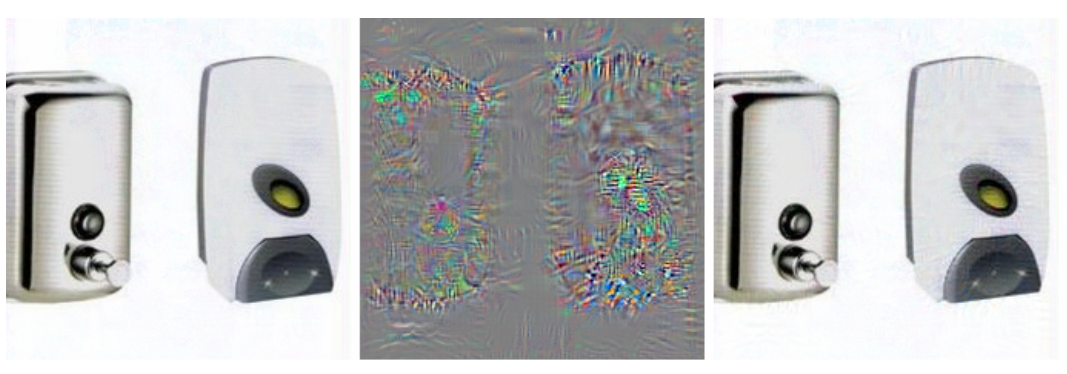
\includegraphics[width=1\textwidth]{graphics/lbfgs.PNG}
    \caption[Example of an adversarial example created by L-BFGS.]{Example of an adversarial example made by L-BFGS \cite{szegedy2014intriguing}. The left image is the original image, which is classified correctly. You can see the adversarial noise in the centre, and on the right you can see the adversarial image, which is classified as an ostrich. Image taken from \cite{szegedy2014intriguing}.}
    \label{fig:lbfgs}
\end{figure}

\begin{figure}[ht]
    \centering
    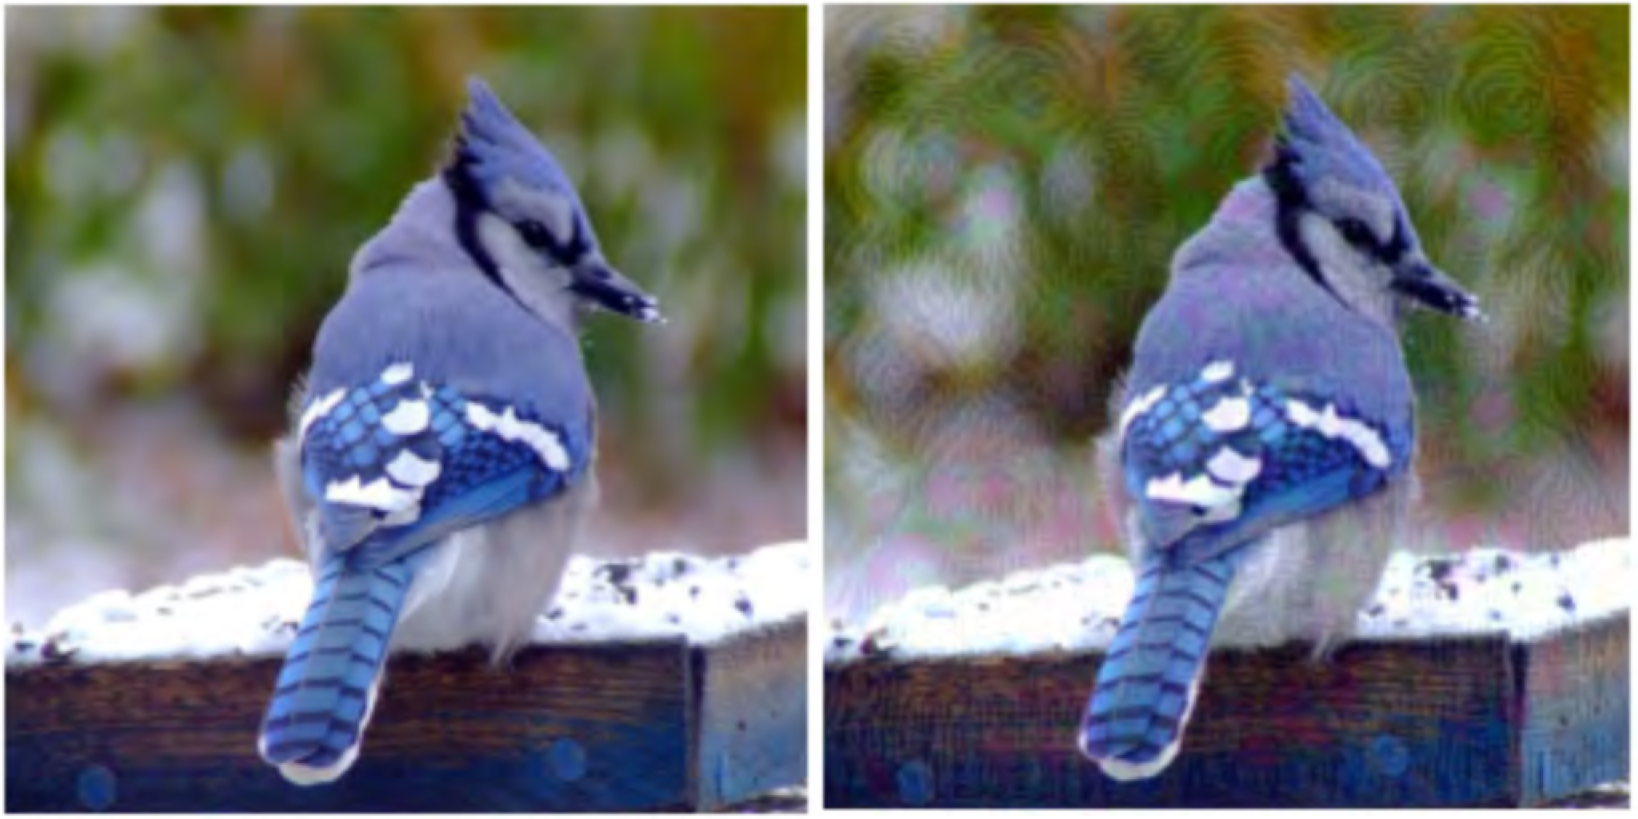
\includegraphics[width=1\textwidth]{graphics/jay_adv_example.PNG}
    \caption[Example of an adversarial example created by \cite{Moosavi-Dezfooli_2017_CVPR}.]{Example of an adversarial example created by the method in \cite{Moosavi-Dezfooli_2017_CVPR}. The left image is the original image of a jay, while the adversarial example on the right is misclassified as a mask. Images taken from \cite{akhtar}.}
    \label{fig:jay_adv_example}
\end{figure}

\subsection{Applicability of adversarial attacks}
  
Ever since the publication of \cite{szegedy2014intriguing}, most of the research has been on CNNs for object recognition tasks \cite{akhtar}. However, adversarial attacks are possible on other architectures, such as GANs \cite{kos_attacks_on_gans}, autoencoders \cite{tabacof_attacks_autoencoders}, recurrent neural networks \cite{papernot_attacks_rnns} and neural networks for semantic segmentation of an image \cite{Metzen_2017_ICCV}. Moreover, autoencoders are much more resilient against adversarial attacks \cite{tabacof_attacks_autoencoders}, and the experiments done by Tang \textit{et al.} \cite{robustart} show that Vision Transformers are more robust against adversarial attacks than CNNs.

\subsection{Transferability of adversarial examples}

Transferability-based black-box attacks succeed due to a property of adversarial examples, first discovered in \cite{szegedy2014intriguing}, that they often manage to fool victim models that are different than the model for which the adversarial example was originally made. This can happen even if the two models have different architectures. Therefore, an attacker can create adversarial perturbations for a substitute model that they control and then use them to mount an attack against another model with inaccessible parameters and loss function gradient. Dong \textit{et al.} \cite{mim} use an optimisation method with momentum to create transferability-based attacks. Meanwhile, ANGRI \cite{upset_angri} is a generative model which learns to create adversarial perturbations by using 3-4 substitute models. Similarly, Zheng \textit{et al.} \cite{zheng_black_box_GAN} train their generator against a substitute model as well.

\subsection{Taxonomy of adversarial attacks}

Silva and Najafirad \cite{silva_survey} categorises attacks based on several criteria. Depending on the \textbf{information} the attacker knows, an attack may be \textbf{white-box} or \textbf{black-box}. In the former, the attacker has full access to the architecture and parameters of the victim model, while in the latter the attacker does not have this knowledge. Dong \textit{et al.} \cite{dong2020benchmarking} further divides black-box attacks into three categories: transferability-based attacks, score-based attacks, where the attacker can query the victim model for soft-label predictions on chosen input, and then estimate the gradient, and decision-based attacks, where the attacker can only query for hard-label predictions, for which it is harder to estimate the gradient.

Attacks can also be classified depending on the \textbf{goals} of the attacker. \textbf{Untargeted} attacks only seek to make the victim model output a wrong result, whatever it may be. Meanwhile, \textbf{targeted} attacks have the goal of making the victim compute a specific wrong label. Furthermore, most attacks produce \textbf{image-specific} perturbations, which are designed to work for one specific image only. However, Moosavi-Dezfooli \textit{et al.} \cite{Moosavi-Dezfooli_2017_CVPR} discovered a method of creating \textbf{universal} adversarial noise, which induces misclassification when applied to the vast majority of images in the dataset. Finally, attacks can be categorised based on the \textbf{attack frequency}, whether the adversarial noise is generated in one step, such as in FGSM \cite{fgsm}, or in an iterative process, like in \cite{carlini2017towards}.

\subsection{Why do adversarial examples exist?}

There are varied and sometimes contradictory viewpoints in regards to why adversarial examples exist and there is no consensus. The hypothesis in Goodfellow \textit{et al.} \cite{fgsm} appears to be the more popular explanation in the literature \cite{akhtar}. This hypothesis says adversarial attacks are caused by the fact that most neural networks are too linear, which is supported by the effectiveness of the FGSM \cite{fgsm} attack method. This excessive linearity could be caused by the popular ReLU activation function, which is piece-wise linear \cite{fgsm}. In Krotov and Hopfield \cite{krotov2018dam}, experiments show that neural networks with highly non-linear activation functions can not be fooled by adversarial examples generated by models equivalent to DNNs with ReLU activation, therefore supporting the linearity hypothesis. 

On the other hand, Tanay and Griffin \cite{tanay2016boundary} contradict this and show that some linear image classifiers are not vulnerable to adversarial attacks. They hypothesize that adversarial examples exist because naturally occurring data samples exist on a subspace of the total input space and that adversarial examples exist when the classification boundary lies too close to this sub-manifold. Therefore, small perturbations manage to move the input across the decision boundary. On the other hand, their experiments show that if the decision boundary is perpendicular to this sub-manifold, the model is more robust against attacks. It is worth noting that their explanation does not totally contradict the linearity hypothesis, as the behaviour they describe is still quite linear.

On a different line of thought, Ilyas \textit{et al.} \cite{adv_examples_bugs} hypothesize that images contain subtle features that are useful for maximising the classification accuracy but are semantically meaningless in regards to the correct label. Adversarial perturbations that resemble these "non-robust" features make the victim model misclassify the adversarial examples with very high confidence.

\subsection{Defences against adversarial attacks}

Defences against adversarial attacks can be classified in the following categories \cite{silva_survey}: gradient masking, used so that the attacker can not use the loss function gradient to create adversarial examples, adversarial example detection and robust optimisation. The latter includes adversarial training, where adversarial examples labelled with the correct label are added to the training set, certified defences, where the model is proven formally to be resistant against perturbations up to a certain limit, and regularisation. The authors of the literature survey in \cite{silva_survey} put a lot of emphasis on certified defences and seem to disregard the effectiveness of adversarial training. However, Dong \textit{et al.} \cite{dong2020benchmarking} performed extensive experiments that show that adversarial training often leads to more robust models than other defences based on regularisation or certified defence.

\section{Adversarial attacks in the physical world}
    \label{sec:physical_attacks_challenges}

Most attacks, including the one in figure \ref{fig:adversarial_segmentation} on page \pageref{fig:adversarial_segmentation}, directly add the perturbations to the whole image. In a realistic setting, the attacker can not directly manipulate the pixels of the input, especially when the model takes its input from sensors. Furthermore, physical adversarial examples, whether 2D printed images or 3D objects, can have their fooling rate diminished by the angle they are viewed from, their distance from the camera, lighting conditions, the inability of the sensor to pick up the subtle adversarial perturbations, and perhaps colour printing errors \cite{kurakin2016adversarial, athalye, evtimov_road_signs}.

Kurakin \textit{et al.} \cite{kurakin2016adversarial} were among the first who investigated adversarial attacks in the physical space. They created adversarial images using FGSM \cite{fgsm}, printed them and took a picture of the printed photos using a smartphone. They then used automatic perspective transformation and cropping to transform the picture, then ran the classifier on it and compared the attack success with the original adversarial example. Over 66.67\% of adversarial examples still fooled the victim model after being printed and photographed. Therefore, it was proven that adversarial examples apply to the physical domain.

However, the photographs taken in \cite{kurakin2016adversarial} only had slight variations in terms of the camera lighting, camera distance and camera angle. Meanwhile, Lu \textit{et al.} \cite{lu_physical_experiments} did similar experiments to the ones in \cite{kurakin2016adversarial}, except they tried a wide variety of camera angles and distances, and they found that the adversarial examples were successful only when the camera was in certain positions. For example, the accuracy of the model doubled or almost tripled when the camera distance increased from 0.5m to 1.5m. Therefore, they concluded that adversarial examples may not be a serious threat to neural networks used in cyber-physical systems.

\subsection{Expectation over Transformation}
    \label{subsec:eot}

To rectify the shortcomings of adversarial attacks mentioned above, Athalye \textit{et al.} \cite{athalye} proposed the Expectation over Transformation (EOT) framework. It is designed to create adversarial examples that are effective in physical settings, and can work on 2D images, 3D rendered objects and 3D printed objects. Their key innovation is that they model transformations such as rotation, translation, perspective projection, 3D rendering or lighting in the optimisation search for the adversarial noise. 

\subsubsection{Technique}
    \label{subsubsec:eot_technique}

The authors optimise the adversarial texture $x^\prime$ in order to maximise the following objective function:

\begin{equation}
\label{eq:eot}
\begin{aligned}
\max_{x^\prime} \quad & \mathrm{E}_{t\sim T}[log P(y_{t} | t(x^\prime))] - \lambda \mathrm{E}_{t\sim T}[d(t(x^\prime), t(x))]\\
\textrm{s.t.} \quad & x \in [0, 1]^d   \\
\end{aligned}
\end{equation}

\noindent where $t(\cdot)$ is a function which simulates the various transformations, $T$ is a distribution of transformation functions, $\lambda$ is a chosen penalty constant, and $d(\cdot, \cdot)$ measures the perceptual difference between x and $x^\prime$.

While $x^\prime$ is the input that the attacker directly controls, $t(x)$ is the input seen by the neural network. In the 3D case, $x$ is a 2D texture and $t(x)$ is a 2D image of a 3D rendered object with that texture, seen from a random angle and distance. You can see an example of this in figure \ref{fig:rendering}. 

\begin{figure}[ht]
    \centering
    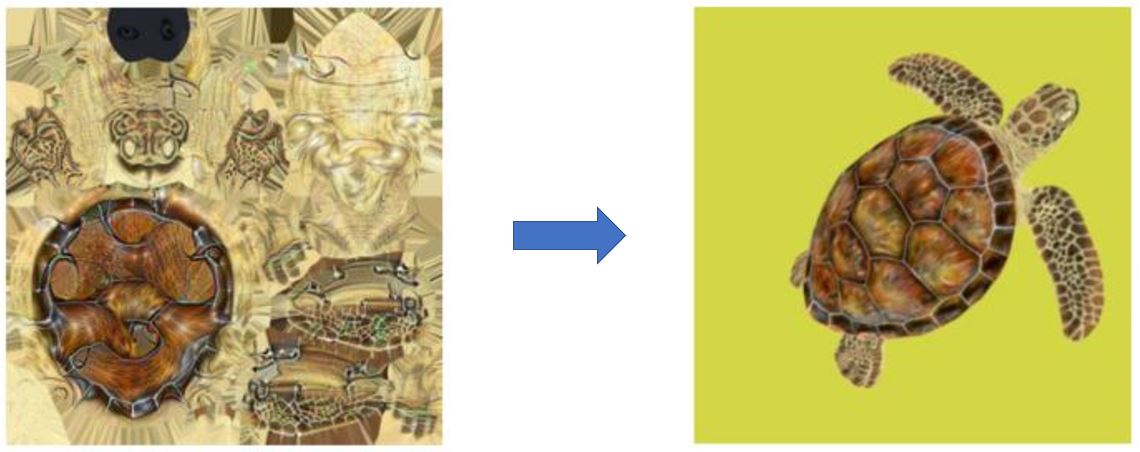
\includegraphics[width=0.8\textwidth]{graphics/rendering.JPG}
    \caption{The transformation function $t(\cdot)$ can model the rendering of a 2D texture into an image of the 3D object with a specific pose. Images are taken from \cite{athalye}.}
    \label{fig:rendering}
\end{figure}

The 3D rendering process is formally considered as a linear transformation such that $t(x) = Mx + b$. This is crucial, because EOT uses gradient descent optimisation, and therefore needs equation \ref{eq:eot} to be differentiable, including the transformation function $t(\cdot)$. The authors of \cite{athalye} claim that the coordinate map $M$ and background $b$ can be calculated for a given object pose by computing the texture-space coordinate for each corresponding on-screen pixel. $M$ and $b$ must be calculated for each new pose of the 3D model. The authors claim that they modified an existing renderer to return this information. However, they do not provide further details on how they compute $M$ and $b$, what they are exactly, nor do they mention which renderer they used. Furthermore, they do not give a link to their source code.

The first term of equation \ref{eq:eot} maximises the log probability that the neural network will classify the adversarial example as the desired target label $y_{t}$. Meanwhile, the second term minimises the distance between the adversarial example and the original input. The authors use the distance function $d(\cdot, \cdot)$ instead of $x^\prime - x$ to focus on the actual perceptual distance between the two, as the classifier sees $t(x)$ rather than $x$.

The framework leaves the choice of the distribution of transformation functions $T$ and the distance function $d(\cdot, \cdot)$ up to the user. According to the supplementary material of Athalye \textit{et al.} \cite{athalye}, the parameters for the camera distance, translation on the x and y axes, rotation of the object, lighting, and 3D printer colour error are each sampled from independent truncated uniform distributions. Camera noise is simulated by using noise drawn from a gaussian distribution.

Meanwhile, the distance metric that they used is the Euclidean distance between the projections in LAB space of $t(x)$ and $t(x^\prime)$. LAB \cite{lab} is a colour space where the Euclidean distance between two colour vectors is roughly equivalent to how different the human eye perceives those colours. The authors chose this metric so that the adversarial noise is less obvious to humans. 

In each optimisation step, the authors use the mean loss function value over a mini-batch of 40 images, each being a different transformation of the same original image. 32 of those are re-used from the previous mini-batch, while the other 8 are new images created with 8 new transformation functions drawn from the distribution $T$. The authors reuse renders as it is computationally expensive to create a new one. By using this process, they ensure that the adversarial object remains adversarial even though it is viewed from a wide variety of perspectives.

\subsubsection{Results and discussion}
    \label{subsubsec:eot_results}

To evaluate the EOT framework for generating 3D adversarial objects, the authors attack an InceptionV3 classifier \cite{inceptionv3} with 78\% accuracy on the Imagenet dataset. For the 3D rendered objects scenario, they used a dataset of 10 3D models, each representing a different class of the Imaganet dataset. For each of these models, they randomly chose 20 random target labels and then created an adversarial texture for that model and target label. 

When evaluating the 200 adversarial examples, they sample 100 random transformations from the distribution $T$ for each example and render 100 images using the adversarial texture and 100 using the original texture. The images with the normal texture had a classification accuracy of 68.8\% and were classified as the adversarial target label 1.1\% of the time. Meanwhile, the adversarial images were classified as the target label 83.4\% of the time, while only 0.01\% of these images were correctly classified.

Following that, Athalye \textit{et al.} created two 3D-printed adversarial objects, a baseball and a turtle, and found that they were classified as the target label 59\% and 82\% of the time, respectively. You can see some photos of the turtle in figure \ref{fig:3d_turtle}. Consequently, we can conclude that the EOT framework can synthesize physical 3D adversarial objects that remain highly effective when viewed from a variety of viewpoints.

Athalye \textit{et al.} \cite{athalye} provides a good high-level description of their proposed framework, and their experiment design is sound. Furthermore, their discussions offer insight into the limitations of their method. However, it lacks some critical information needed to re-create their work. As mentioned in subsection \ref{subsubsec:eot_technique}, they do not explain exactly how to get the necessary parameters to represent $t(\cdot)$ as a linear transformation, nor do they provide a link to their source code or even the data set they used. Furthermore, they do not mention what optimiser learning rate or penalty constant $\lambda$ they used or for how many steps they ran their algorithm. Finally, a step-by-step algorithm would have been useful for implementing EOT and re-creating their results.

\begin{figure}[ht]
    \centering
    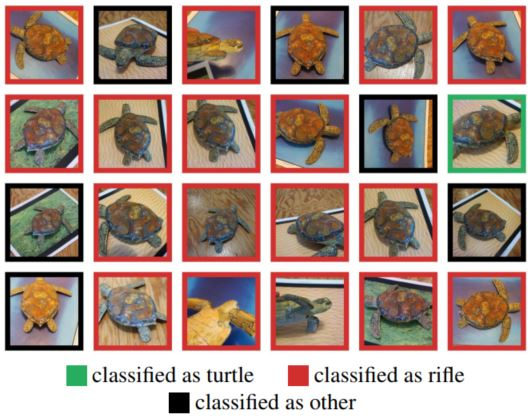
\includegraphics[width=1\textwidth]{graphics/turtle.JPG}
    \caption{A selection of photographs of the 3D adversarial turtle object. The adversarial perturbation was made for the "rifle" target label. Taken from \cite{athalye}.}
    \label{fig:3d_turtle}
\end{figure}

\subsection{Robust Physical Perturbations}

Concurrently to Athalye \textit{et al.} \cite{athalye}, Eykholt \textit{et al.} \cite{evtimov_road_signs} developed an attack for 2D physical objects, such as traffic signs, called Robust Physical Perturbations ($\textrm{RP}_2$).

\subsubsection{Technique}

In contrast with EOT \cite{athalye}, where the transformation functions from $T$ synthetically augmented the dataset by rendering the 3D object in various poses, here the authors augment it by manually taking photos of the original object from various angles and distances and in varying lighting conditions. They further use some synthetic transformations in the form of cropping and changing the image brightness to add new transformed images to the dataset. The input to $\textrm{RP}_2$ is a photo of an object taken from its front, and during the optimisation process, it draws a new sample from a distribution $X$ of images of that same object, seen under various transformations.

Moreover, because the input to $\textrm{RP}_2$ is an image of the physical 3D object rather than a 2D texture of an object, the authors use a mask $M_x$ to make sure that the adversarial perturbation $\delta$ is only applied to object itself and not to the image background. The mask is a matrix the size of the image, with a 0 for each pixel where no perturbation should be added, and 1 otherwise. 

With these changes in mind, the authors of \cite{evtimov_road_signs} define the optimisation problem in $\textrm{RP}_2$ as:

\begin{equation}
\begin{aligned}
\min_{\delta} \quad & \lambda\|M_x \cdot \delta\|_p + NPS + \mathrm{E}_{x_i\sim X}J(f_\theta(x_i + T_i(M_x \cdot \delta)), y_t)\\
\label{eq:rp2}
\end{aligned}
\end{equation}

\noindent where $NPS$ is a term for correcting printing colour errors, $J(\cdot, \cdot)$ is the loss function of the classifier represented by $f_\theta$, $y_t$ is the adversarial target label and $T_i$ is a function that transforms the perturbation to match the object in the image. If the object is seen from a 30\degree{} angle, the perturbation is rotated by 30\degree{} in 3D. The first term is for minimising the size of the perturbation, and the third term ensures that the adversarial example is misclassified.

\subsubsection{Results and discussion}
    \label{subsubsec:rp2_results}

Eykholt \textit{et al.} used $\textrm{RP}_2$ to create a poster of a road STOP sign, with perturbations applied to the whole surface of the sign. They manually took photos of the poster from a variety of distances and angles and fed them into a CNN trained on the LISA traffic sign dataset. 100\% of those photos were misclassified as the target label by the network, with an average confidence of 80.51\%. In another experiment, they created adversarial patches in the form of stickers and placed them over a STOP sign. Just like in the previous experiment, they took photos of the sign and then fed them into the LISA CNN. The attack with regular stickers had a 100\% success rate, and an attack with a sticker which looked like graffiti succeeded 66.67\% of the time. Finally, they put adversarial stickers over a real STOP sign on a street and took photos of it from a moving car. The attack success rate was 92.4\%, once more proving the effectiveness of their algorithm.

$\textrm{RP}_2$ is an interesting attack method which is capable of producing robust adversarial examples for road signs, thus endangering traffic safety. However, it is quite inconvenient. It requires the user to manually take a lot of photos and manually create the perturbation mask $M_x$. Furthermore, the authors of \cite{evtimov_road_signs} do not offer any detailed information on how the perturbation alignment function $T_i$ works, not even in the supplementary material. Finally, their approach is only applicable to flat physical surfaces, like road signs. On the other hand, EOT works for any 3D object \cite{athalye}, and could also use a mask to create adversarial patches like \cite{evtimov_road_signs} did.

\section{Generative Models for black-box attacks}
    \label{sec:generative_models}
    
\subsection{Generator-simulator model}
    \label{subsec:zheng}

Zheng \textit{et al.} \cite{zheng_black_box_GAN} proposed a generative model for creating targeted black-box adversarial examples for 2D images. Its architecture consists of two components, a generator and a simulator. The purpose of the simulator is to act as a substitute for the black-box victim model, while the generator creates adversarial noise for a given image and target label.

\subsubsection{Technique}

The simulator is trained so that it provides the same output as the victim model for a given adversarial example created by the generator:

\begin{equation}
\begin{aligned}
\min_{\theta_s} \quad & L(S(\theta_s, x + G(x, z)),V(\theta_v, x + G(x, z)))\\
\textrm{s.t.} \quad & x \in X, \|G(x, z)\|_\infty < \delta
\label{eq:simulator_loss}
\end{aligned}
\end{equation}

\noindent where the outputs predicted by the simulator and victim model are denoted by $S(\cdot,\cdot)$ and $V(\cdot,\cdot)$, respectively. $\theta_s$ and $\theta_v$ are the parameters of the simulator and victim model, respectively. The adversarial noise created by the generator for a given image $x$ and a given target label $z$ is written as $G(x,z)$. $X$ is the training set and $\delta$ is the perturbation budget. $L(\cdot,\cdot)$ represents the cross-entropy loss function. Equation \ref{eq:simulator_loss} is visualised in figure \ref{fig:zheng_simulator_loss}. It is essentially a simplified version of distillation \cite{distillation}.

\begin{figure}[ht]
    \centering
    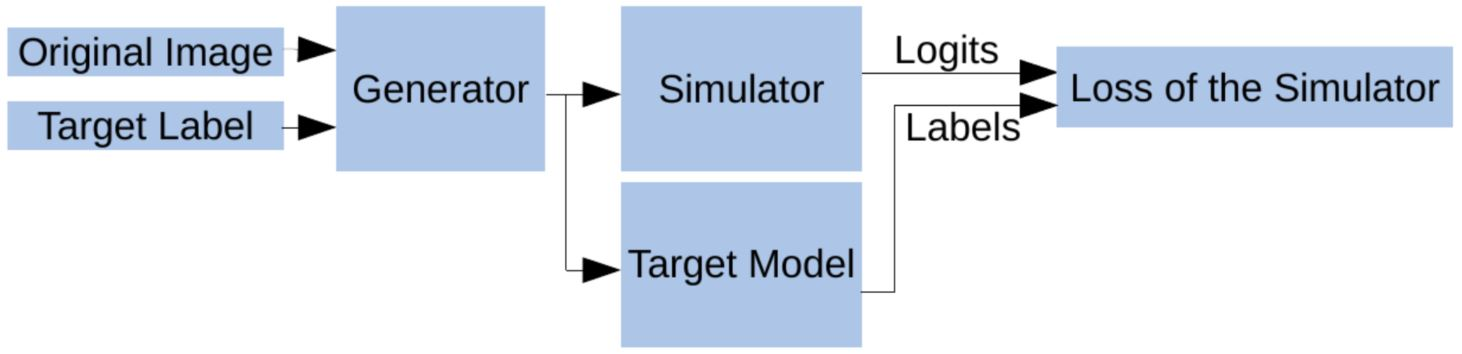
\includegraphics[width=1\textwidth]{graphics/simulator_loss.JPG}
    \caption{Computational flow of the loss function for training the simulator. Diagram taken from \cite{zheng_black_box_GAN}.}
    \label{fig:zheng_simulator_loss}
\end{figure}

Meanwhile, the generator is trained to fool the simulator such that the latter will classify the generated adversarial image with the desired wrong label $z$. Training the generator takes the following form:

\begin{equation}
\begin{aligned}
\min_{\theta_g} \quad & L(S(\theta_s, x + G(x, z)),z) + \beta\|G(x,z)\|_2\\
\textrm{s.t.} \quad & x \in X, z \in Y \setminus \{y\}\\
\label{eq:generator_loss}
\end{aligned}
\end{equation}

\noindent where $\theta_g$ is the parameter vector of the generator, $Y$ is the set of labels and $y$ is the correct label of $x$. $\beta$ is a constant for the perturbation size penalty. The first term of equation \ref{eq:generator_loss} maximises the probability that the simulator will classify the generator output as the target label, while the second term constrains the $\ell_2$ norm of the noise image vector.  Figure \ref{fig:zheng_generator_loss} visualises the generator training process.

\begin{figure}[ht]
    \centering
    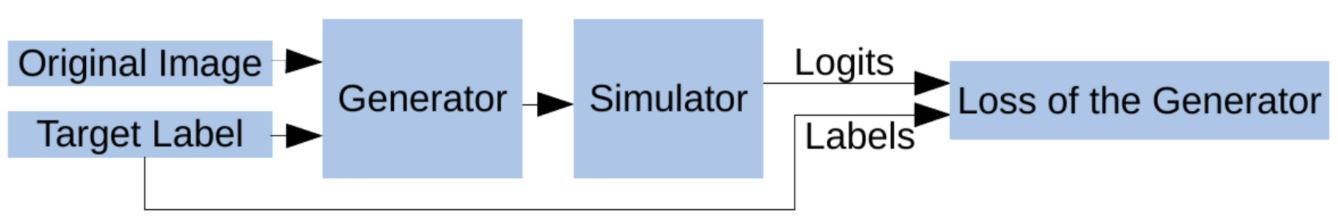
\includegraphics[width=1\textwidth]{graphics/generator_loss.JPG}
    \caption{Computational flow of the loss function for training the generator. Diagram taken from \cite{zheng_black_box_GAN}.}
    \label{fig:zheng_generator_loss}
\end{figure}

The simulator in the paper is a CNN. The proposed generator is an auto-encoder, as you can see in figure \ref{fig:zheng_generator}. The encoder takes the form of a CNN without fully connected layers or global average pooling, and its job is to encode an image as a vector in higher-dimensional latent space. 

\begin{figure}[ht]
    \centering
    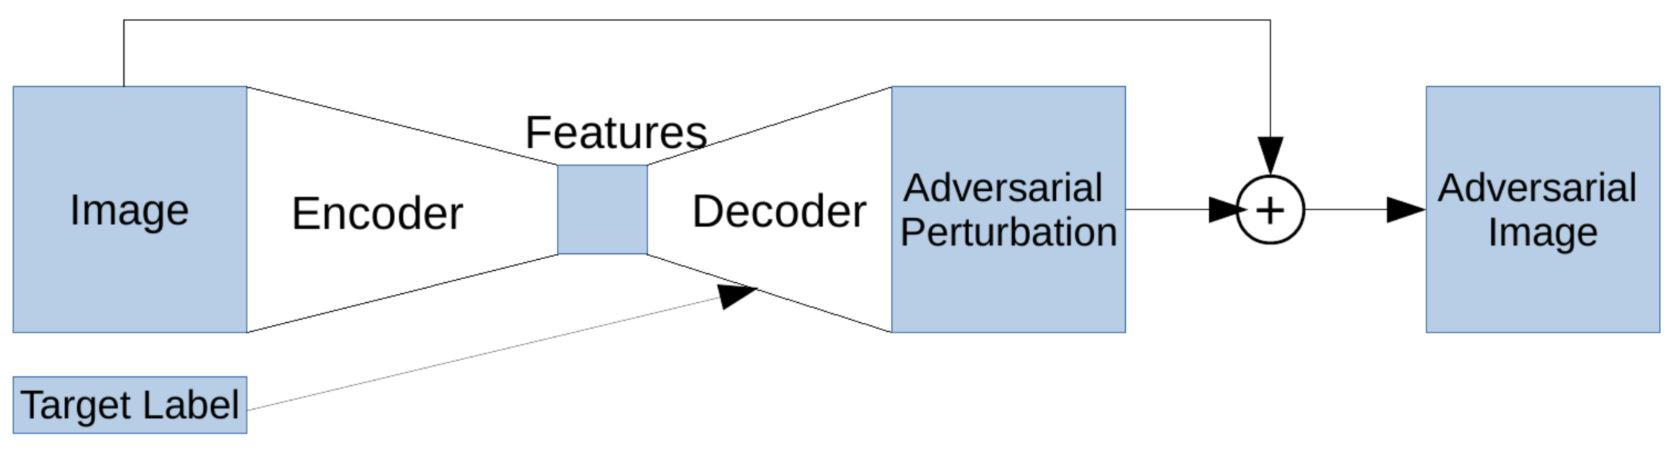
\includegraphics[width=1\textwidth]{graphics/generator.JPG}
    \caption{The autoencoder architecture of the generator in \cite{zheng_black_box_GAN}. Diagram taken from \cite{zheng_black_box_GAN}.}
    \label{fig:zheng_generator}
\end{figure}

The decoder is an ensemble of neural networks made out of transposed convolution layers, as you can see in figure \ref{fig:zheng_decoder}. It uses an ensemble because the perturbation must be designed for a given target label. The decoder has a gating sub-network inspired by Shazeer \textit{et al.} \cite{experts_mixture_gate} which learns to create a sparse weights vector based on the target label. This sub-network is just one fully connected layer with as many output neurons as there are experts. The output of the decoder is a weighted sum of the outputs of each expert model, using the weights from the gating network. Different combinations of expert models are used for different target labels, and each expert learns to focus on one or a couple of target labels.

\begin{figure}[ht]
    \centering
    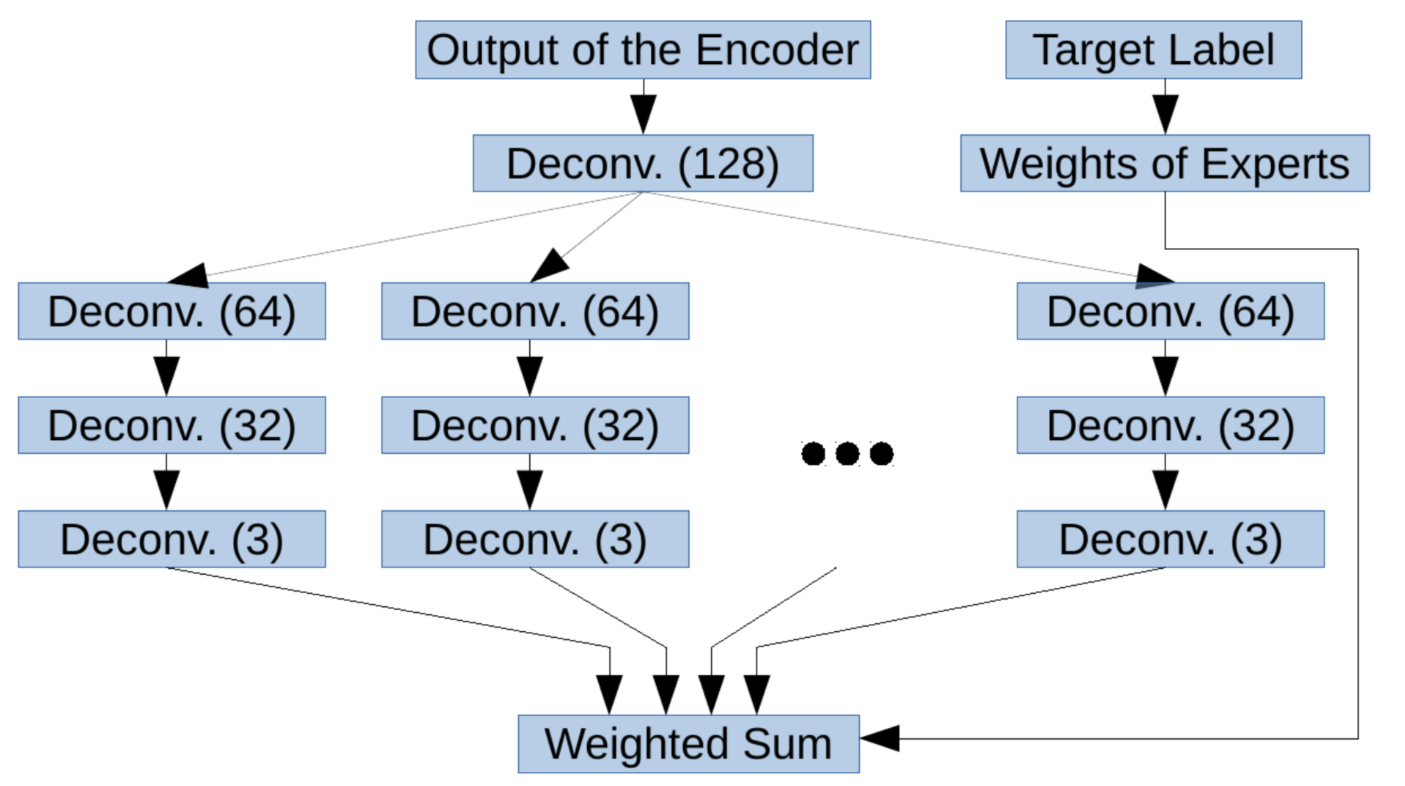
\includegraphics[width=0.8\textwidth]{graphics/decoder.PNG}
    \caption{The decoder architecture of the generator in \cite{zheng_black_box_GAN}. Diagram taken from \cite{zheng_black_box_GAN}.}
    \label{fig:zheng_decoder}
\end{figure}

The authors train the simulator and generator in alternative steps. Moreover, the authors used a number of techniques to improve results and speed-up training. Before the main training loop, they warm-up the simulator by training it on normal images. During the main loop, they also train the simulator on images with random noise, and not just with adversarial noise. Furthermore, they clip the gradients of the generator to values between -1 and 1.

\subsubsection{Results and discussion}

Zheng \textit{et al.} \cite{zheng_black_box_GAN} evaluate their model on the CIFAR-10 dataset and experiment with 4 different CNNs as simulators. These include 3 small novel CNNs, SmallNet, SimpleNet and ConcatNet, with architectures inspired by ResNet \cite{resnet}, Xception \cite{xception} and DenseNet \cite{densenet} respectively. The fourth is the Xception model \cite{xception} itself. They try all 16 possible combinations of the 4 CNNs as both simulator and victim model, with an average success rate of over 80\% across the 16 experiments and with a minimum of 63\% and a maximum of 87.3\%. Considering that all 4 CNNs had an accuracy of over 90\% on normal images, this demonstrates that the proposed technique can effectively create black-box attacks on CIFAR-10 CNNs. Moreover, it outperforms the attack success rate of the earlier generative model made by Sarkar \textit{et al.} \cite{upset_angri}. The authors repeated their experiments on CIFAR-100, where they had an attack success rate of 72.1\%.

The paper demonstrates an effective method to create a generator for black-box adversarial attacks on small images and provides plenty of details to enable someone to re-create their work. The diagrams of the model architecture are very clear, and the authors provide values for most hyper-parameters. However, they do not mention how long they trained their model, nor what learning rate, optimiser and batch size they used, and the paper does not have supplementary material. They do not provide a link to their source code either.

\subsection{AdvGAN}
    \label{subsec:AdvGAN}
    
Concurrently with Zheng \textit{et al.} \cite{zheng_black_box_GAN}, Xiao \textit{et al.} \cite{advGAN} created a generative adversarial network (GAN) \cite{gans} to create adversarial images in the black-box setting. It is similar to the former, and therefore this subsection will concentrate on the differences between the two.

\subsubsection{Technique}

AdvGAN has a generator network which produces adversarial noise and a simulator which is trained to behave like the black-box victim model, just like Zheng \textit{et al.} does. However, it also uses a discriminator, as you can see in figure \ref{fig:advgan}, where the simulator is called a "distilled black-box". 

\begin{figure}[ht]
    \centering
    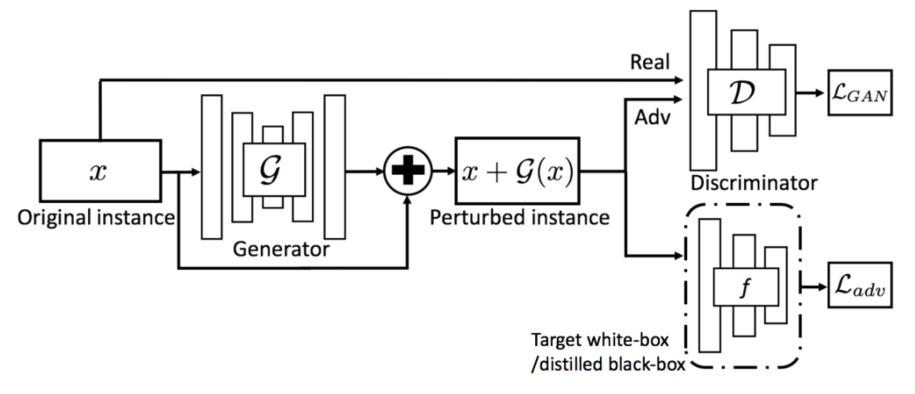
\includegraphics[width=0.8\textwidth]{graphics/advgan.PNG}
    \caption{High-level overview of AdvGAN. Diagram taken from \cite{advGAN}.}
    \label{fig:advgan}
\end{figure}

Unlike in \cite{zheng_black_box_GAN}, the generator trains to fool the discriminator into thinking adversarial images are normal images, while also training to fool the simulator into classifying the adversarial images as the desired target label. Meanwhile, the discriminator trains to tell if an image contains noise made by the generator. The generator training against the discriminator ensures that the adversarial noise is hard to distinguish. The noise is further constrained by a hinge loss:

\begin{equation}
\begin{aligned}
\mathrm{L}_\textrm{hinge} = \mathrm{E}_x max(0, \|G(x)\|_2 - c)\\
\label{eq:advgan_hing_loss}
\end{aligned}
\end{equation}

which adds a penalty if the Euclidean length of the noise vector is under $c$, while Zheng \textit{et al.} simply used an $\ell_2$ penalty term.

The simulator is trained to behave like the victim model using distillation \cite{distillation}. After every step of training the generator and discriminator, the simulator performs a training step with both normal and adversarial images as input. On the other hand, Zheng \textit{et al.} \cite{zheng_black_box_GAN} only do so with adversarial images and trains the simulator on normal images only during the initial warm-up phase.

The discriminator of AdvGAN is a CNN which performs binary classification on patches of the input image and then averages the patch predictions to determine if the whole image is adversarial. The generator is an auto-encoder where the encoder is made up of convolutional layers, while the decoder is made of transposed convolutions. Unlike in the generator of Zheng \textit{et al.}, AdvGAN has pairs of encoder and decoder layers with residual connections between them, as U-Net does \cite{unet}. Finally, the generator of AdvGAN does not make use of a mixture-of-experts in its decoder, and therefore it can not generate perturbations for all target labels and must be re-trained for each target label. This is in contrast with the generator in subsection \ref{subsec:zheng}, which could generate adversarial examples for any target label.

\subsubsection{Results and discussion}

The authors evaluate AdvGAN against ResNet-32 and Wide ResNet-34 \cite{resnet} models trained on CIFAR-10, and in the black-box setting the targeted attack has a success rate of 78.5\% and 81.8\%, respectively. Moreover, it achieved an attack success rate of 92.76\% in the black-box setting of the MadryLab challenge \cite{madrylab}. Finally, the authors claim that they managed to create adversarial noise for 100 high-resolution ImageNet-like images against an InceptionV3 model \cite{inceptionv3} with a 100\% attack success rate.

Xiao \textit{et al.} created a powerful generative network for targeted black-box attacks, and the paper provides a lot of detail on the overview of the model and on how it is trained. Moreover, it performs a wide range of experiments, with both white-box and black-box settings, as well as attacking models with defences against adversarial attacks. However, they do not provide detailed information on the exact architecture they used for the discriminator and generator, they just say "adopt similar architectures for generator and discriminator with image-to-image translation literature" then cite two papers. They do not provide source code or supplementary material either. However, the largest downside of their model is that it must be trained for each individual target label.

Furthermore, their claim of a 100\% attack success rate on high-resolution images is odd, as they do not mention how they adapted their architecture for larger input, and it makes no sense how the attack was even more successful than against simpler models on CIFAR-10. The example Imagenet adversarial images in the paper look identical to the normal images, too.

	\chapter{Methodology}
    \label{chap:methodology}
    
In this chapter, we will be discussing the research methodology of the project, then explain the implementation of the proposed model and the metrics which will be used in experiments.

As you will see later in section \ref{sec:proposed_model}, our proposed model is a combination of the methods of \cite{athalye} and \cite{zheng_black_box_GAN}, and therefore it is necessary to implement those papers and re-create some of the results of those papers to ensure these implementations are correct, before merging the two for our own model. Therefore, we will cover these implementations in sections \ref{sec:eot_implementation} and \ref{sec:zheng_implementation}.
    
\section{Research methodology}

The EOT framework presented in subsection \ref{subsec:eot} is highly effective at creating robust adversarial noise for 3D-rendered objects. This is despite the fact it is training on renders of the object with a random position and angle. In EOT, the transformation from the texture to the rendered image is represented as a simple linear transformation. At the same time, generative models have proven to be capable at learning a distribution for generating large 256x256 images \cite{big_gan}, especially benefiting from having significantly more parameters. Therefore, my intuition is that with the proper training hyper-parameters and architecture, a generative model should be able to learn to create adversarial textures. Since the transformation representing 3D rendering is linear, it should not be an insurmountable obstacle for training the generator.

Moreover, the black-box generative model in subsection \ref{subsubsec:zheng} can be easily combined with the EOT framework for making adversarial objects in subsection \ref{subsec:eot}, by placing a differentiable rendering pipeline between the generator and the simulator.

\newpage
The research hypothesis of this project is the following: 

\textit{It is possible to use a generative neural network to create 3D-rendered adversarial objects in the targeted black-box setting that have a targeted fooling rate of at least 50\% on a victim CNN classifier for object recognition.}

\bigbreak
The targeted fooling rate metric is explained later in section \ref{sec:analytic_techniques}.

This is a quantitative experimental research project. The model proposed in section \ref{sec:proposed_model} creates 3D-rendered objects, and pictures of those objects will be given to various neural network classifiers. The predicted label will be compared against the correct label and the adversarial target label to evaluate the effectiveness of the proposed method. We will mainly be using a circulatory research process, to try Further details on the experiments are found in subsection \ref{sec:experiment_design}.

\section{Implementation of EOT}
    \label{sec:eot_implementation}

Like subsection \ref{subsec:eot} mentioned, the authors of \cite{athalye} fail to include detailed information into how they represented 3D rendering as a differentiable linear transformation. One of the authors provides a step-by-step guide with source code \cite{athalye_step_by_step}, but only for attacks for 2D images, not for textures which are then rendered as 3D objects. I therefore searched Github.com for repositories related to \cite{athalye}, and found one implementation of the paper for the 3D rendered objects case \cite{ring_adversarial_3d}. 

However, the implementation lacked documentation and was written in Tensorflow 1, which is obsolete, less intuitive and harder to debug. I forked the repository and almost completely re-wrote the code to run with Tensorflow 2 \footnote{Source code at https://github.com/Alexandru-Dascalu/adversarial-3d}, documented it and refactored it according to software engineering principles, although the algorithm is broadly the same as \cite{ring_adversarial_3d} implemented it.

\subsection{UV mapping}

3D models are made up of a series of vertices, points in 3D space which define the shape of an object. To apply a texture to a model, one method is to use UV coordinates, which are pairs of coordinates which tell you which pixel from the texture image should be used to colour a certain vertex. These coordinates are defined when the 3D model is created, and come included with the vertex coordinates in the 3D model file. After rendering a 3D model, an OpenGL renderer will look up the UV coordinates for each vertex, and for each triangle it will copy the fragment of the texture that is within the three texture coordinates of the triangle, thus creating a textured object. A UV map is what Athalye \textit{et al.} \cite{athalye} likely referred to when talking about texture-space coordinates.

A normal renderer will take the array of vertices, the UV map and the object's texture as inputs. It will first render the object by translating and rotating the position vector of each vertex \cite{opengl_shaders}. Following that, it will use the UV coordinates of each vertex to sample a colour from the texture, either by using nearest-neighbour, bilinear interpolation or anisotropic filtering \cite{opengl_textures}. However, the renderer implemented by \cite{ring_adversarial_3d} and used by us simply returns the UV coordinates instead of a colour. Therefore, the output of the renderer is a 299x299 image of the object rendered in the desired pose, but instead of a colour with RGB values, each pixel has a U and V coordinate pointing to a pixel in the texture. We are going to call this output image a "UV map" from now on.

The renderer is implemented using ModernGL \footnote{https://github.com/moderngl/moderngl}, a Python wrapper around OpenGL which allows you to render .obj files with textures.

\subsection{Transformation from texture to image}
    \label{subsec:eot_transformation}
    
\begin{algorithm}
\caption{Pseudo-code representation of the transformation function $t(\cdot)$}
\label{alg:rendering}
\begin{algorithmic}[1]
\STATE $std\_textures \gets repeat(std\_texture)$
\STATE $adv\_textures \gets repeat(adv\_texture)$
\IF{print\_error}
    \STATE $std\_textures, adv\_textures \gets apply\_print\_error(std\_textures, adv\_textures)$
\ENDIF
\STATE $std\_image \gets resample(std\_textures, uv\_maps)$
\STATE $adv\_images \gets resample(adv\_textures, uv\_maps)$

\STATE $std\_images, adv\_images \gets add\_background(std\_textures, adv\_textures)$

\IF{photo\_error}
    \STATE $std\_images, adv\_images \gets apply\_photo\_error(std\_images, adv\_images)$
\ENDIF

\STATE $std\_images, adv\_images \gets normalise(std\_images, adv\_images)$
\RETURN $std\_images, adv\_images$
\end{algorithmic}
\end{algorithm}

The renderer produces a UV map for each image in the mini-batch, which together with the texture is used as input for the algorithm seen in algorithm \ref{alg:rendering}. This algorithm is a step-by-step representation of the $t(x) = Mx + b$ function mentioned in section \ref{subsubsec:eot_technique}. As we will see, this algorithm is indeed just a linear transformation. The reason that this algorithm creates images with both the original and adversarial paper is that we need to calculate difference between them for the penalty term in equation \ref{eq:eot} on page \pageref{eq:eot}. Since this penalty seeks to measure the perceptual difference caused by the adversarial noise, all other parameters such as the pose of the object or the background colour must identical for each pair made up of a normal and an adversarial image.

The $repeat(\cdot)$ function in lines 1 and 2 of the pseudocode simply replicates the 3D texture tensor as many times as the size of the batch, as you can see in listing \ref{lst:repeat}.

\lstinputlisting[language={python}, label={lst:repeat}, caption={An implementation of the repeat function from algorithm \ref{alg:rendering}}]{./listings/repeat.py}

\lstinputlisting[language={python}, label={lst:print_error}, caption={Simulating 3D printer errors.}]{./listings/print_error.py}

Athalye \textit{et al.} \cite{athalye} modelled per-colour channel 3D printer errors in their experiments with 3D-printed adversarial objects. The $apply\_print\_error$ function implements this by randomly generating a scalar multiplier and addend for each colour channel in each batch texture, and using those to linearly transform the texture, as you can see in listing \ref{lst:print_error}.

After applying the print error, we can create the batch of 299x299 images of the rendered object. The $resample(\cdot, \cdot)$ function from algorithm \ref{alg:rendering} is implemented as the $resampler(\cdot, \cdot)$ method from the tensorflow\_addons library \cite{tfa_resampler}. For each pixel in each image, it samples a colour from that image's texture based on the UV coordinates of the corresponding pixel in that image's UV map. tensorflow\_addons.resampler uses bilinear interpolation to mix the colours of neighbouring texture pixels to get the colour it will return \cite{tfa_resampler}. Therefore, it is a linear transformation.

\lstinputlisting[language={python}, label={lst:add_background}, caption={Code for adding colour background to the renders of the 3D object.}]{./listings/background.py}

In \cite{athalye}, the authors used random colours for the background of each render. Therefore, for each image we compute a mask with true boolean values for each pixel that makes up the object. The UV maps have a value of 0 for each pixel that makes up the background of the scene rather than the object, so we just check for UV coordinates different than 0. We then sample an RGB colour from a truncated uniform distribution. We obtain the background by performing element-wise multiplication between the colour vector and a logical inverse of the mask, which has true values for the background and false for the object. We then add that with a multiplication between each image with its mask, which essentially "cuts out" the rendered object and adds it on top of the background. This process can be seen in code listing \ref{lst:add_background}.

Since a 3D-printed adversarial object would be photographed with a camera connected to a neural network, Athalye \textit{et al.} \cite{athalye} also modelled random lighting conditions and camera noise in their experiments with physical objects. Our implementation, represented by the $apply\_photo\_error(\cdot, \cdot)$ function in algorithm \ref{alg:rendering}, linearly scales each image with a random scalar multiplier and addend to lighten or darken the image. It then simulates camera noise by adding gaussian noise.

\lstinputlisting[language={python}, label={lst:normalise}, caption={Source code for normalising the rendered images}]{./listings/normalise.py}

Finally, the $normalise(\cdot, \cdot)$ function from algorithm \ref{alg:rendering} linearly normalises the images, as the random scaling done when applying the photo or print error may result in values outside $[0, 1]$. Firstly, we calculate the minimum and maximum pixel values across all colour channels for each image. We will then pick the minimum and maximum values for each pair of normal and adversarial images. This is important, as the adversarial noise may fall outside $[0, 1]$, and because it is semantically meaningful, the normal image must use the linear scale as its adversarial counterpart. Finally, if a minimum or maximum value is inside $[0, 1]$, we set it to 0 or 1, respectively. This is because scaling is done only to bring invalid values inside the valid range. This normalisation process can be seen in code listing \ref{lst:normalise}.

\subsection{Creating the adversarial texture}

The rest of the implementation works just how subsection \ref{subsubsec:eot_technique} described the EOT framework \cite{athalye}. Rendered images of the 3D model are created using the algorithm described in subsection \ref{subsec:eot_transformation}. As seen in the code listings in subsection \ref{subsec:eot_transformation}, these renders are dependent on parameters drawn from uniform distributions for the rotation, camera distance, X/Y translation, print error, lighting, camera noise and background colour.

The rendered images are given to the victim model for inference. The resulting logits, together with the target labels, are used to calculate the average cross-entropy loss across all images in the mini-batch. This is the first term of the objective function in equation \ref{eq:eot} on page \pageref{eq:eot}. Furthermore, we calculate the second term of that equation by projecting the normal and adversarial images into LAB space \cite{lab} using the scikit-image library \footnote{https://scikit-image.org/docs/dev/api/skimage.color.html\#skimage.color.rgb2lab}, then calculating the average $\ell_2$ norm of the difference between each of pair of normal and adversarial images. An Adam optimiser is used to update the adversarial texture such that the objective function in equation \ref{eq:eot} is minimised.

At each optimisation step, a certain percentage of rendered images from the previous mini-batch are re-used, as Athalye \textit{et al.} also did. This is implemented by shifting the previous tensor of images to the left, thus discarding some of the images from the previous mini-batch, then adding the new renders at the end. Therefore, old renders are gradually replaced. For example, with a re-use percentage of 80\%, there is an entirely new batch of renders after every 5 optimisation steps. For added efficiency, the logits of the victim model for old renders are memorised rather than re-calculated at each stop, logits are computed only for the new renders.

\section{Implementation of Zheng et al.'s model}
    \label{sec:zheng_implementation}
    
I searched Github.com for an existing implementation of Zheng \textit{et al.} \cite{zheng_black_box_GAN}, and found a Tensorflow implementation made by the authors of the paper themselves \footnote{https://github.com/StanleyZheng-FDU/targeted-black-box-attack}. Unfortunately, it was also written in Tensorflow 1, lacked documentation and had a lot of duplicate or unused code. On the other hand, it implemented all models and training techniques described by Zheng \textit{et al.} \cite{zheng_black_box_GAN}.

Due to time constraints, I chose not to completely re-write this implementation in Tensorflow 2. I forked the repository \footnote{https://github.com/Alexandru-Dascalu/targeted-black-box-attack} and only added some comments, some minor refactors to improve code readability and some code to plot the training history.

\section{Proposed model for G-EOT}
    \label{sec:proposed_model}
    
\subsection{Overview}
    \label{subsec:g_eot_overview}

The proposed G-EOT model is at a high level the same generative model presented in subsection \ref{subsubsec:zheng}, except that it has elements of the EOT framework \cite{athalye} added to it. The key difference is that the generator produces adversarial perturbations for a 2D texture rather than an image of an object, as you can see in figure \ref{fig:architecture}. The perturbations are then added to the original texture to create the adversarial texture. The latter is then rendered as a 3D object, and an image of the rendered object is then given to the simulator and to the victim model.

\begin{figure}[h]
    \centering
    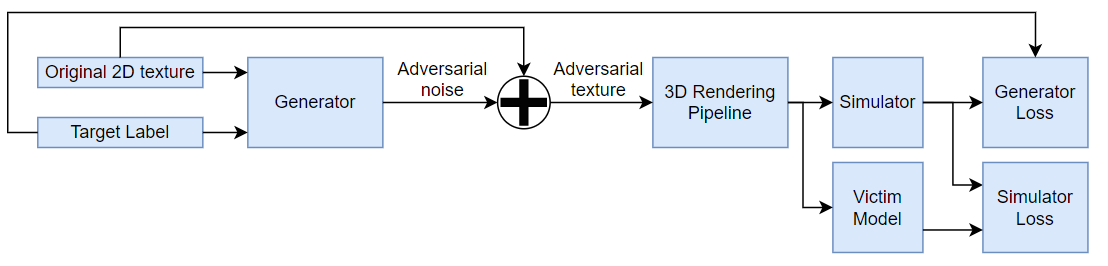
\includegraphics[width=1\textwidth]{graphics/architecture.PNG}
    \caption{The architecture of G-EOT.}
    \label{fig:architecture}
\end{figure}

The 3D rendering pipeline in figure \ref{fig:architecture} is essentially identical to the one presented in section \ref{sec:eot_implementation}. It simulates 3D rotation, translation, varying camera distance, different background colours and lighting conditions, camera noise, and 3D printer error. The parameters for 3D rendering are sampled from truncated uniform distributions, similarly to the distribution $T$ of transformation functions presented in the supplementary material of \cite{athalye}. 

All textures for 3D models that I could find had at least 1024x1024 pixels, with most having a resolution of 2048x2048. Since generative models struggle to generate output larger than 256x256 pixels \cite{big_gan}, the generator first performs average pooling on the texture to reduce its resolution. The adversarial noise created by the generator has a resolution of 256x256. This is then upsampled using bilinear interpolation to 2048x2048 pixels so that it can be added to the original texture to obtain the adversarial texture.

\begin{wrapfigure}[27]{r}{0.3\textwidth}
    \centering
    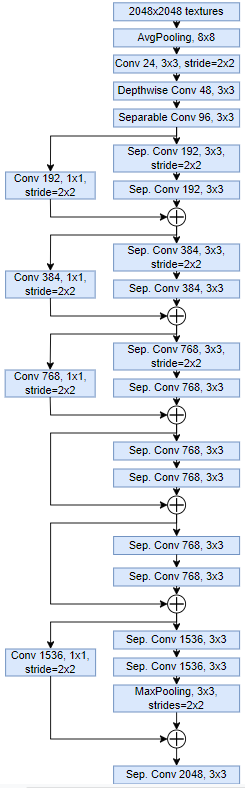
\includegraphics[width=0.3\textwidth]{graphics/g_eot_encoder.PNG}
    \caption{The structure of the encoder in the G-EOT generator.}
    \label{fig:proposed_encoder}
\end{wrapfigure}

EOT \cite{athalye} was chosen rather than $\textrm{RP}_2$ \cite{evtimov_road_signs} because it is a lot more convenient, for reasons named in subsection \ref{subsubsec:rp2_results}. Furthermore, the synthetic transformation functions for 3D rendered objects can accurately simulate real-world transformations \cite{athalye}. On the other hand, the method presented in Zheng \textit{et al.} \cite{zheng_black_box_GAN} was chosen for the genera-simulator model rather than one from Xiao \textit{et al.} \cite{advGAN} because it is simpler and it can generate attacks for all target labels, as mentioned in subsection \ref{subsec:AdvGAN}.

\subsection{Generator}

The generator is an auto-encoder with a similar structure as the one in figure \ref{fig:zheng_generator} in subsection \ref{subsubsec:zheng}. Its encoder is a CNN with an architecture inspired by the SimpleNet CNN from Zheng \textit{et al.} \cite{zheng_black_box_GAN}, which is itself inspired by Xception \cite{xception}. 

Its structure can be seen in figure \ref{fig:proposed_encoder}. The numbers after the type of the convolutional layer are the number of output channels of that layers, followed by the kernel size. Although not seen in the diagram, each convolutional layer is followed by a batch normalisation layer \cite{batch_norm}.

Meanwhile, the structure of the decoder is exactly the same as the one in Zheng \textit{et al.} \cite{zheng_black_box_GAN}, shown in figure \ref{fig:zheng_decoder} on page \pageref{fig:zheng_decoder}. A more detailed diagram of the generator is in appendix \ref{app:detailed_architecture}.

The loss function used to train the generator is the same as equation \ref{eq:generator_loss} on page \pageref{eq:generator_loss} describes, except that it is not enough for the penalty term to be the $\ell_2$ norm of the adversarial noise, as the victim model does not perceive the texture directly, but rendered images of the 3D model instead. Therefore, the penalty term used is:

\begin{equation}
    \label{eq:g-eot-l2-loss}
    \begin{aligned}
    \beta\|t(x + G(x,z)) - t(x)\|_2
    \end{aligned}
\end{equation}

\noindent where $x$ is the original texture, $z$ is the target label, $t(\cdot)$ is the transformation function represented by the 3D rendering pipeline, and $G(\cdot, \cdot)$ is the adversarial noise created by the generator. The image with the adversarial texture and the image with the normal texture use the same function $t(\cdot)$ so that the images will have the same pose, and the only difference is caused by the perceived adversarial noise. I chose not to project the images into LAB space, as Athalye \textit{et al.} did, to simplify the training task of the generator.

\subsection{Simulator}

\begin{wrapfigure}[24]{r}{0.3\textwidth}
    \centering
    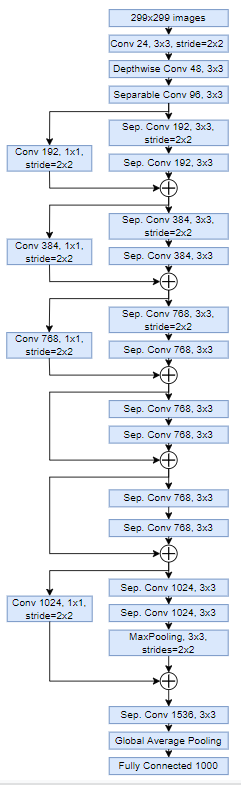
\includegraphics[width=0.3\textwidth]{graphics/g_eot_simulator.PNG}
    \caption{The structure of the G-EOT simulator.}
    \label{fig:proposed_simulator}
\end{wrapfigure}

The simulator is also a CNN inspired by the SimpleNet architecture from Zheng \textit{et al.} \cite{zheng_black_box_GAN}, and it is almost identical to the architecture of the encoder, though its last three convolutional layers have fewer kernels, and it has a global average pooling and a fully connected layer at the end, and it does not have the average pooling layer at the beginning. It can be seen in figure \ref{fig:proposed_simulator}, and a more detailed diagram is in appendix \ref{app:detailed_architecture}.

Moreover, the loss function for training the simulator is the same as equation \ref{eq:simulator_loss} from subsection \ref{subsubsec:zheng}. 

\subsection{Training techniques}
    \label{subsec:training}

Firstly, the simulator is warmed up by training it to predict the same labels as the victim model does on images rendered using normal textures. This is done to speed-up training, as Zheng \textit{et al.} \cite{zheng_black_box_GAN} explained.

Following that, the simulator and generator are trained in alternative steps. In each simulator training steps, two steps are actually performed to train the simulator to imitate the victim model. In the first one, the simulator and victim model are given as input images rendered with normal textures. In the second one, they are given images with textures perturbed by the generator. This is done to ensure that throughout training, the simulator further learns to be an accurate imitation of the black-box victim model.

Then a training step is performed for the generator. It trains to generate adversarial noise for textures such that images rendered with those textures fool the simulator, as described by equation \ref{eq:generator_loss} in subsection \ref{subsubsec:zheng} and in subsection \ref{subsec:g_eot_overview}. The gradients of the generator loss function are clipped before they are applied, just as Zheng \textit{et al.} \cite{zheng_black_box_GAN} did for their model.

Unlike in Athalye \textit{et al.} \cite{athalye}, no renders are re-used between mini-batches. This is done because it has been observed that the maximum batch size for G-EOT that can fit in 8GB of memory is only 5. Generating 5 new renders for each training step can be done fast enough, and the model trains better the more new unique samples it sees.

\section{Analytic techniques}
    \label{sec:analytic_techniques}
    
Unless otherwise specified, each experiment will use the following metrics to evaluate the proposed attack's success:

\begin{itemize}
    \item \textbf{Targeted Fooling Rate (TFR):} the percentage of adversarial examples that are classified by the victim model as the desired target label. Please note that TFR is the same thing as the adversariality metric used in Athalye \textit{et al.} \cite{athalye}. It is also frequently called "attack success rate" in the literature.
    \item \textbf{Untargeted Fooling Rate (UFR):} the percentage of adversarial examples that are classified by the victim model as any incorrect label. It is relevant because if the attack induces a misclassification, even if it is not the desired target label, then it is still potentially dangerous.  It is always equal to $1 - accuracy$.
    \item \textbf{Classification Accuracy:} the percentage of adversarial examples classified with the correct label. It is always equal to $1 - UFR$.
\end{itemize}

	\chapter{Results and discussion}
    \label{chap:results}

\section{Dataset}
    \label{sec:dataset}
    
The data set is made up of 15 3D models, each one representing a different object which has a class in the ImageNet dataset. Each model consists of a 2D texture, a .obj file, and a text file. The .obj file contains the vertices making up the 3D object and and each vertex's texture coordinates, while the text file contains a list of correct labels.

All 3D models and their textures were obtained by manually searching 3D asset sites for suitable models, and were not created by me. All credits for the models go to their respective creators, seen in Appendix \ref{app:model_credits}. Each model was manually re-scaled using the Blender 3D graphics tool \footnote{https://www.blender.org/} such that all 15 models are of comparable size. This was done to ensure that each model would not need different rendering parameter distributions to properly fit into the rendered image.

Out of the 15 models, 10 represent the same classes that the dataset of 10 3D models used by Athalye \textit{et al.} \cite{athalye} also represented. This was done in order to properly reproduce the experimental results of Athalye \textit{et al.}. Please keep in mind that these 10 models are not the same ones that Athalye \textit{et al.} used, as they did not publish their dataset. The other 5 models represent other ImageNet classes: a crocodile, a killer whale, a jeep, a running shoe and a rugby ball.

You can view the correct labels for each model in table \ref{table:model_labels_accuracy}, along with the classification accuracy of InceptionV3 on rendered images of each model.

The choice of suitable models were constrained by the following requirements:

\begin{itemize}
    \item The model has to be free.
    \item It has to have a texture, not a solid colour.
    \item It has to have only one texture, not multiple ones for different parts of the object, as the renderer only applies one texture to the object.
    \item Rendered images of the model must be classified accurately by a pre-trained InceptionV3 classifier at least 30\% of the time.
    \item The model must not have transparent surfaces such as car windows, as the implemented renderer can not calculate UV coordinates for that surface.
\end{itemize}

Due to the above requirements, I could not find a very good 3D model for a taxi. The one I settled for has a different texture for its wheels and license plates, and the renderer simply applies parts of the main texture for the body of the taxi to the wheels, making them look yellow, as you can see in figure \ref{fig:taxi}. Similarly, a suitable model for a sofa, as used by Athalye \textit{et al.} \cite{athalye}, could not be found. Several models that were tried were classified correctly by an InceptionV3 classifier less than 10\% of the time. Therefore, a 3D model of a purse is used instead.

\begin{figure}[ht]
    \centering
    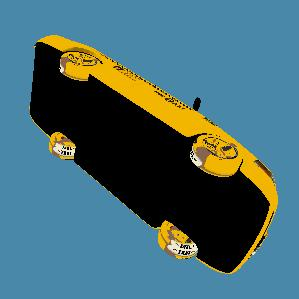
\includegraphics[width=0.4\textwidth]{graphics/taxi.jpg}
    \caption{A render of the taxi model with its original texture. As you can see, the renderer applies parts of the car body texture to the wheels.}
    \label{fig:taxi}
\end{figure}

The original textures of the model had a resolution of 1024x1024, 2048x2048 or 4096x496 pixels. Since the generator requires a each input texture to have the same size, the 4096x4096 textures were downsampled to 2048x2048 using OpenCV's resize function with INTER\_AREA interpolation \footnote{https://learnopencv.com/image-resizing-with-opencv/}. The 1024x1024 pixels textures were upsampled to 2048x2048 pixels using OpenCV's resize function with bicubic interpolation.

Some models have multiple correct labels for two reasons. The first one is that a pre-trained InceptionV3 \cite{inceptionv3} model consistently misclassifies some rendered objects with the same wrong labels, but those labels are semantically related to the correct class. For example, the purse model is often confused with a wallet, but since both a purse and a wallet are made of the same material and have similar colours, we consider this to be meaningful. Similarly, the jeep model is frequently misclassified as a "half-track" and as an "amphibious vehicle", both of those being somewhat similar to jeeps. Secondly, some 3D models can fit in a variety of Imagenet classes. The model of a muscle car can be reasonably described as both a "sports car" and a "race car".

\begin{table}
\caption{The 3D model dataset, with the correct labels of each model, and the classification accuracy of InceptionV3 on 100 rendered images of those models.}
\label{table:model_labels_accuracy}
\begin{tabular}{|p{2.6cm} | p{8.5cm}| p{2cm}|} 
 \hline
 Model Name & Labels & Classification Accuracy (\%) \\
 \hline
 barrel & barrel/cask (427) & 92.8 \\ 
 \hline
 baseball & baseball (429) & 100 \\
 \hline
 camaro & station wagon (436), race car (751), sports car (817) & 10.8 \\
 \hline
 clownfish & anemone fish (393) & 37.2 \\
 \hline
 crocodile & African crocodile (49), American alligator (50) & 44  \\
 \hline
 german\_shepherd & All 118 dog breeds (labels 151 to 268), as well as grey wolf, white wolf, red wolf, coyote, dingo, dhole, hyena dog (labels 269 to 275) & 73.2 \\
 \hline
 jeep & amphibious vehicle (408), half-track (586), jeep (609) & 19 \\
 \hline
 orange & orange (950) & 59 \\
 \hline
 orca & orca (148) & 69 \\
 \hline
 purse & purse (748), wallet (893) & 71 \\
 \hline
 rugby\_ball & rugby ball (768) & 95 \\
 \hline
 running\_shoe & running shoe (770) & 35 \\
 \hline
 sea\_turtle & loggerhead turtle (33), leatherback turtle (34), mud turtle (35), terrapin (36), box turtle (37) & 89.8 \\
 \hline
 taxi & taxi (468) & 15 \\
 \hline
 teddy & teddy bear (850) & 54 \\
 \hline
\end{tabular}
\end{table}


\section{EOT for rendererd 3D objects}

\subsection{Experiment Design}
    \label{subsec:eot_experiment_design}

To validate that our implementation of EOT is correct, we evaluate if the attack success rate is the same as Athalye \textit{et al.} \cite{athalye} reported on their experiments with adversarial examples for 3D rendered objects. For each 3D model, Athalye \textit{et al.} chose 20 random target labels and used EOT to create adversarial textures. Then for each of these 200 textures, they sampled 100 different random poses and rendered images of the 3D model in that pose and with the adversarial texture. These images were fed into Tensorflow's pre-trained InceptionV3 classifier neural network, and the authors measured how often they were classified with the correct label versus the adversarial label.

The procedure used by me is similar. I use 10 out of the 15 models in the dataset, the ones matching the models used by Athalye \textit{et al.}, and for each one 5 target labels are sampled from a uniform distribution, ensuring that they are different to the correct labels. Only 5 target labels are used instead of 20 due to computational and time constraints.

The EOT implementation described in section \ref{sec:eot_implementation} is used to create 50 adversarial textures.  Tensorflow Keras's pre-trained InceptionV3 neural network is used again to evaluate rendered images of the adversarial objects. The algorithm is run until the average loss of the past 400 steps is below 0.5, or for 10000 steps at most. A constant learning rate of 0.003 is used. 

Just as it was done in \cite{athalye}, 80\% of samples from the current mini-batch are re-used in the next mini-batch. For models whose original texture was 1024x1024, I chose to use that rather than the texture upscaled to 2048x2048 pixels, as a smaller texture allows for a larger batch sizes, which gives better results. The batch size is 40 for models with 1024x1024 textures, the same batch size used in \cite{athalye}. For textures with 2048x2048 pixels, the batch size is 30, the maximum that 8GB of memory can fit. 

The authors of \cite{athalye} say that for each model/target label pair they tried four values for the $\lambda$ hyper-parameter from equation \ref{eq:eot} on page \pageref{eq:eot}, used for constraining perceptual difference between normal and adversarial images. They then chose the adversarial example that had the best attack success rate. They do not say what value they used for each adversarial example. Due to time and computation constraints, it was unfeasible to try 4 different $\lambda$ values for each of the 50 adversarial examples. Some ad-hoc experiments done with the crocodile 3D model indicates that a value of 0.025 ensures that the adversarial texture looks similar to the original one, while not still having a high attack success rate. Therefore, this was used for the EOT implementation evaluation.

The rendering parameters are sampled from uniform distributions identical with those used by Athalye \textit{et al.} \cite{athalye}, which you can see in table 2 of their supplementary material. Translation on the X/Y axes is quit small, between -0.05 and 0.05. The rotation angle on all three axes is drawn from an unbounded uniform distribution. The camera distance is between 1.8 and 2.3, while in \cite{athalye} it was between 2.5 and 3. The reason behind this is that the 3D models in my dataset appear to be smaller than those used in \cite{athalye}, and so the camera distance was reduced to make them appear to the camera as large as they did in Athalye \textit{et al.}. You can see in figure \ref{fig:barrel_comparison} that with the adjusted camera distance, the barrel model appears roughly as large as the model used in \cite{athalye}. Finally, because this experiment is on evaluating EOT on 3D rendered objects and not physical 3D printed adversarial objects, printer and camera errors are not modelled, and the apply\_print\_error and apply\_photo\_error functions from algorithm \ref{alg:rendering} on page \pageref{alg:rendering} are not called.

\begin{figure}[H]
\centering
\subfloat[Model used in \cite{athalye}.]{
	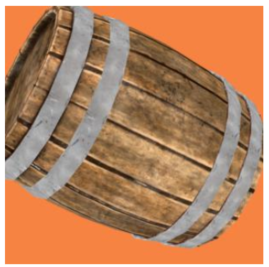
\includegraphics[width=0.4\linewidth]{./graphics/athalye_barrel.png}
}~ % Use a tilde to add spacing for sub-figures that are displayed next to one another horizontally.
\subfloat[Model used by this project.]{
	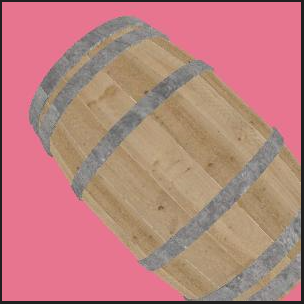
\includegraphics[width=0.4\linewidth]{./graphics/my_barrel.png}
}\\ % New line before caption.

\caption[Comparison of the camera distances used in Athalye \textit{et al.} versus this project.]{A comparison of an image of the barrel model used in Athalye \textit{et al.} versus an image of the barrel model used by this project.}
\label{fig:barrel_comparison}
\end{figure}

After creating the 50 adversarial textures, the same renderer used during the EOT optimisation process is used to create the evaluation images. For each adversarial texture, 100 images of the rendered object with that texture are created. For each image with the adversarial texture, an image of the object in the same pose and with the same background colour, but with the normal texture, is rendered. You can see an example of this in figure \ref{fig:evaluation_images_comparison}. This is done to observe the effect of using the adversarial texture rather than the original one, as all other factors are the same.

\begin{figure}[H]
\centering
\subfloat[Adversarial image.]{
	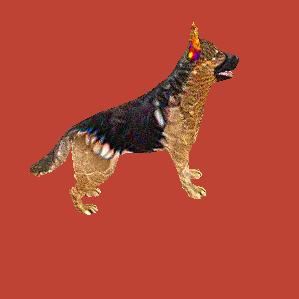
\includegraphics[width=0.485\linewidth]{./graphics/adv_dog_image.jpg}
}~ % Use a tilde to add spacing for sub-figures that are displayed next to one another horizontally.
\subfloat[Normal image.]{
	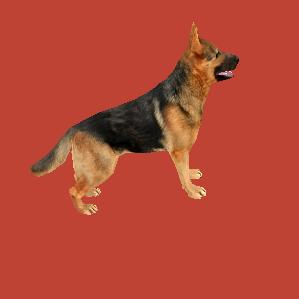
\includegraphics[width=0.485\linewidth]{./graphics/std_dog_image.jpg}
}\\ % New line before caption.

\caption[Comparison between equivalent adversarial and normal images for evaluation.]{Comparison between an evaluation image of the dog model with the adversarial texture versus its normal counterpart. The adversarial texture is for the "black grouse" target label.}
\label{fig:evaluation_images_comparison}
\end{figure}

\subsection{Experiment Results}
    \label{subsec:eot_experiment_results}

On the 5000 images with the normal textures, the average classification accuracy was 60.28\%, while only 0.08\% of them were classified as the adversarial target label. By comparison, the 20000 normal images in Athalye \textit{et al.} \cite{athalye} had an accuracy of 68.8\% and only 0.01\% were classified as the target label. These figures are similar, although my images had a significantly lower classification accuracy. This is caused by the low classification accuracies for normal images of the taxi and camaro models being only 15 and 10.8, as you can see in table \ref{table:model_labels_accuracy}. Without these two models, the average accuracy would be 72.125\%. 

But on the adversarial images, the average classification accuracy was just 0.86\%, very close to the EOT paper's result of 1.1\% \cite{athalye}. Meanwhile, the average TFR was 80.08\%, slightly under the TFR of 83.4\% seen in the EOT paper. The slightly worse performance may be caused by a multitude of factors. Even though the dataset described in section \ref{sec:dataset} is designed to mimick the one used in \cite{athalye}, it is not identical. Furthermore, different values for the $\lambda$ penalty constant, learning rate, and number of steps were used compared to \cite{athalye}, as the authors did not specify what values they used. The mean TFR and the target labels for each individual model can be seen in table\ref{table:eot_results}.

The fact that the adversarial textures brought down the classification accuracy from 60.28\% to 0.86\%, and increased the TFR from 0.08\% to 80.08\%, demonstrates the this implementation of EOT \footnote{https://github.com/Alexandru-Dascalu/adversarial-3d} is highly effective at creating robust adversarial attacks for 3D rendered objects. Moreover, the results are very similar to those in \cite{athalye}, demonstrating that it is an accurate re-creation of the implementation used by the authors of that paper.

In figure \ref{fig:eot_histogram} you can see a histogram of the TFR for each of the 50 adversarial textures. You can see that 27 out of 50 adversarial textures had a mean TFR of over 90\%. Meanwhile, just 2 adversarial textures are failures, with a a mean TFR under 20\%. This demonstrates that the vast majority of adversarial textures for 3D objects are highly successful.

\begin{figure}[ht]
    \centering
    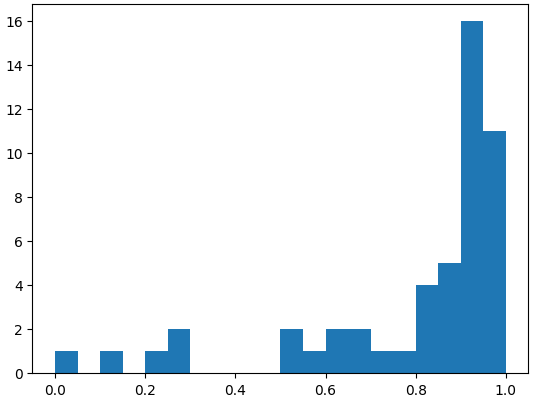
\includegraphics[width=0.7\textwidth]{graphics/eot_histogram.PNG}
    \caption{Histogram of TFR of the 50 adversarial examples.}
    \label{fig:eot_histogram}
\end{figure}

It took 82 hours to create the 50 adversarial textures on an RTX 3070 with 8GB of VRAM. That GPU can do around 2900 EOT optimisation steps in an hour, and therefore the creation of a single adversarial texture can take up to around 3.4 hours.

All 50 adversarial textures created by and used in this experiment can be seen in appendix \ref{app:adversarial_textures}.

\begin{table}
\caption{Results of the EOT experiment on rendered 3D objects.}
\label{table:eot_results}
\begin{tabular}{|p{2.6cm} | p{6.5cm} | p{2cm}| p{2cm}|} 
 \hline
 Model Name & Target Labels & Mean TFR (\%) & Mean number of iterations \\
 \hline
 barrel & file cabinet, hourglass,hautboy, purse, typewriter keyboard & 95.59 & 1428.4 \\ 
 \hline
 baseball & australian terrier, dingo, indian elephant, radiator, warplane & 80.6 & 6349.2 \\
 \hline
 camaro & kite, mongoose, indri, trombone, red-breasted merganser & 93.39 & 2585.8 \\
 \hline
 clownfish & swimming cap, grand piano, shopping basket, wall clock, bridegroom & 48.2 & 10000 \\
 \hline
 german\_shepherd & bald eagle, barrel, bikini, black grouse, hornbill & 85.6 & 5243 \\
 \hline
 orange & whippet, goblet, lighter, missile, plate & 97.4 & 1163.2 \\
 \hline
 purse & pit bull terrier, chickadee, dhole, weevil, sandbar & 42.8 & 9090.6 \\
 \hline
 sea\_turtle & Australian terrier, leopard, mantis, cradle, plunger & 80.39 & 5123 \\
 \hline
 taxi & groenendael, marmot, acoustic guitar, cradle, radiator grille & 87.8 & 4229.6 \\
 \hline
 teddy & soft-coated wheaten terrier, leatherback turtle, pool table, hot pot, pineapple & 89 & 2782.8 \\
 \hline
\end{tabular}
\end{table}

\newpage
\subsection{Discussion}

\subsubsection{Classification accuracy on normal images}

The very low InceptionV3 classification accuracies for normal texture images of the taxi and camaro models of 15 and 10.8 percent, respectively, might be caused by the fact that the objects are rendered with completely random rotations on the X, Y and Z axes. Therefore, these cars are often seen from below or above. The images of taxis or sports cars in the Imagenet dataset are of cars as they appear on the street, and therefore seen from the side or from the front or back, not from above or underneath.

Then again, the classification accuracy on images with the nomal texture does not seem to impact the performance of EOT. The adversarial textures for taxi and camaro models had a mean TFR of 87.8\% and 93.39\%, respectively.

\subsubsection{EOT performance depending on the model}

Out of the two adversarial textures with a mean TFR of under 20\%, one is the adversarial texture for the clownfish model and the grand piano target label, the other is the one for the purse model and the pit bull terrier label. Even without those two, the mean TFRs of the clownfish and purse adversarial textures are around only 50\%. The ability of EOT to create adversarial examples seems to be influenced by the perceptual difference between the model and the target label. A clownfish has a vastly different shape and colour to a piano. In particular, the colour pattern of a clownfish is very distinct, and likely prevents the renders of the adversarial clownfish to be classified as a piano. It would require many more optimisation steps to distort it so it has piano features on it.

Similarly, the brown purse model has a very different colour to a pit bull terrier, resulting in the TFR of 0.1\% for that model. However, the purse adversarial texture for the Asian wild dog target label had a mean TFR of 62\%. The contrast may be explained by the fact that the wild dog is brown in colour, and thus already perceptually closer to the brown purse.

Models with a simple shape, similar to a sphere, and/or a colour pattern dominated by one simple colour, seem to be a better "canvas" for EOT to apply adversarial noise to. The barrel and orange 3D models have a mean TFR of over 90\%, as you can see in table \ref{table:eot_results}. The camaro and taxi models mostly have a solid yellow colour and they have a mean TFR of over 85\%. On the other hand, models with more complicated shapes like the sea turtle and the german shepherd have a lower mean TFR. 

A simple colour ensures that EOT can gradually develop adversarial patterns more easily, while a simpler shape means that the model looks similar regardless of the angle it is viewed from, which makes the gradient fluctuate less despite the random poses the models are rendered in.

\subsubsection{Number of iterations}

As subsection \ref{subsec:eot_experiment_design} mentioned, the algorithm stopped when the average loss of the past 400 steps was below 0.5, or for at most 10000 steps. Table \ref{table:eot_results} displays the average number of iterations it took to create the five adversarial examples for each model. It is likely that that threshold for stopping the algorithm could have been set to 0.8 instead of 0.5 to reduce runtime, while obtaining similar TFRs.

Unsurprisingly, the models with the lowest mean TFR, the clownfish and the purse, also took the longest to create. Meanwhile, the models with a simpler texture and colour were easier to optimise. For example, it took EOT on average just 1163.2 iterations to run for the orange model. 

The number of necessary optimisation steps is influenced by the somewhat random nature of the gradient, caused by the fact that each rendered image in the batch is random. This perceptual randomness is smaller for models with a simple shape, as they look similar regardless of the angle they are seen from. As you can see in figure \ref{fig:eot_orange_loss_history}, the loss value fluctuates much less for the orange model, leading to a much faster convergence. At the other extreme, the loss value for the clownfish model and shopping basket target label fluctuates wildly, sometimes from a value of 1 to 3 or even 4, as you can see in figure \ref{fig:eot_clownfish_loss_history}. The "Main loss" in these loss history plots refer to the value of the first term in equation \ref{eq:eot} in subsection \ref{subsubsec:eot_technique}, while "L2 Loss" refers to the penalty constraining the size of the adversarial perturbation in that equaton. "Total Loss" refers to the sum of these terms.

\begin{figure}[ht]
    \centering
    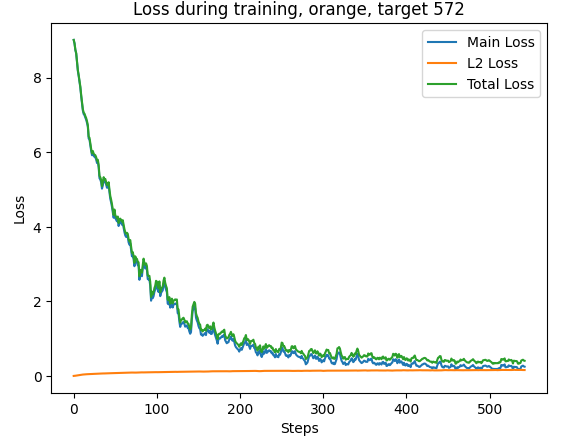
\includegraphics[width=0.7\textwidth]{graphics/eot_orange_loss_history.PNG}
    \caption{Optimisation history for the orange model and target label goblet. L2 loss refers to the penalty term in equation \ref{eq:eot}, main loss refers to the first term. Its evaluation TFR is 100\%.}
    \label{fig:eot_orange_loss_history}
\end{figure}

\begin{figure}[ht]
    \centering
    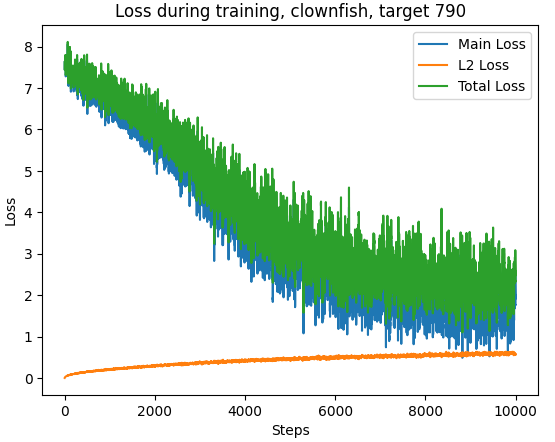
\includegraphics[width=0.7\textwidth]{graphics/eot_clownfish_loss_history.PNG}
    \caption{Optimisation history for the clownfish model and target label shopping basket. Its TFR is 71\%.}
    \label{fig:eot_clownfish_loss_history}
\end{figure}

Another interesting observation is that the longer the EOT algorithm has to run, the more noisy the created adversarial textures will be. You can see this in the textures in figures  \ref{fig:clownfish_noisy_texture} and \ref{fig:dog_noisy_texture}, both which took the maximum number of 10000 steps to create,

\begin{figure}[H]
    \centering
    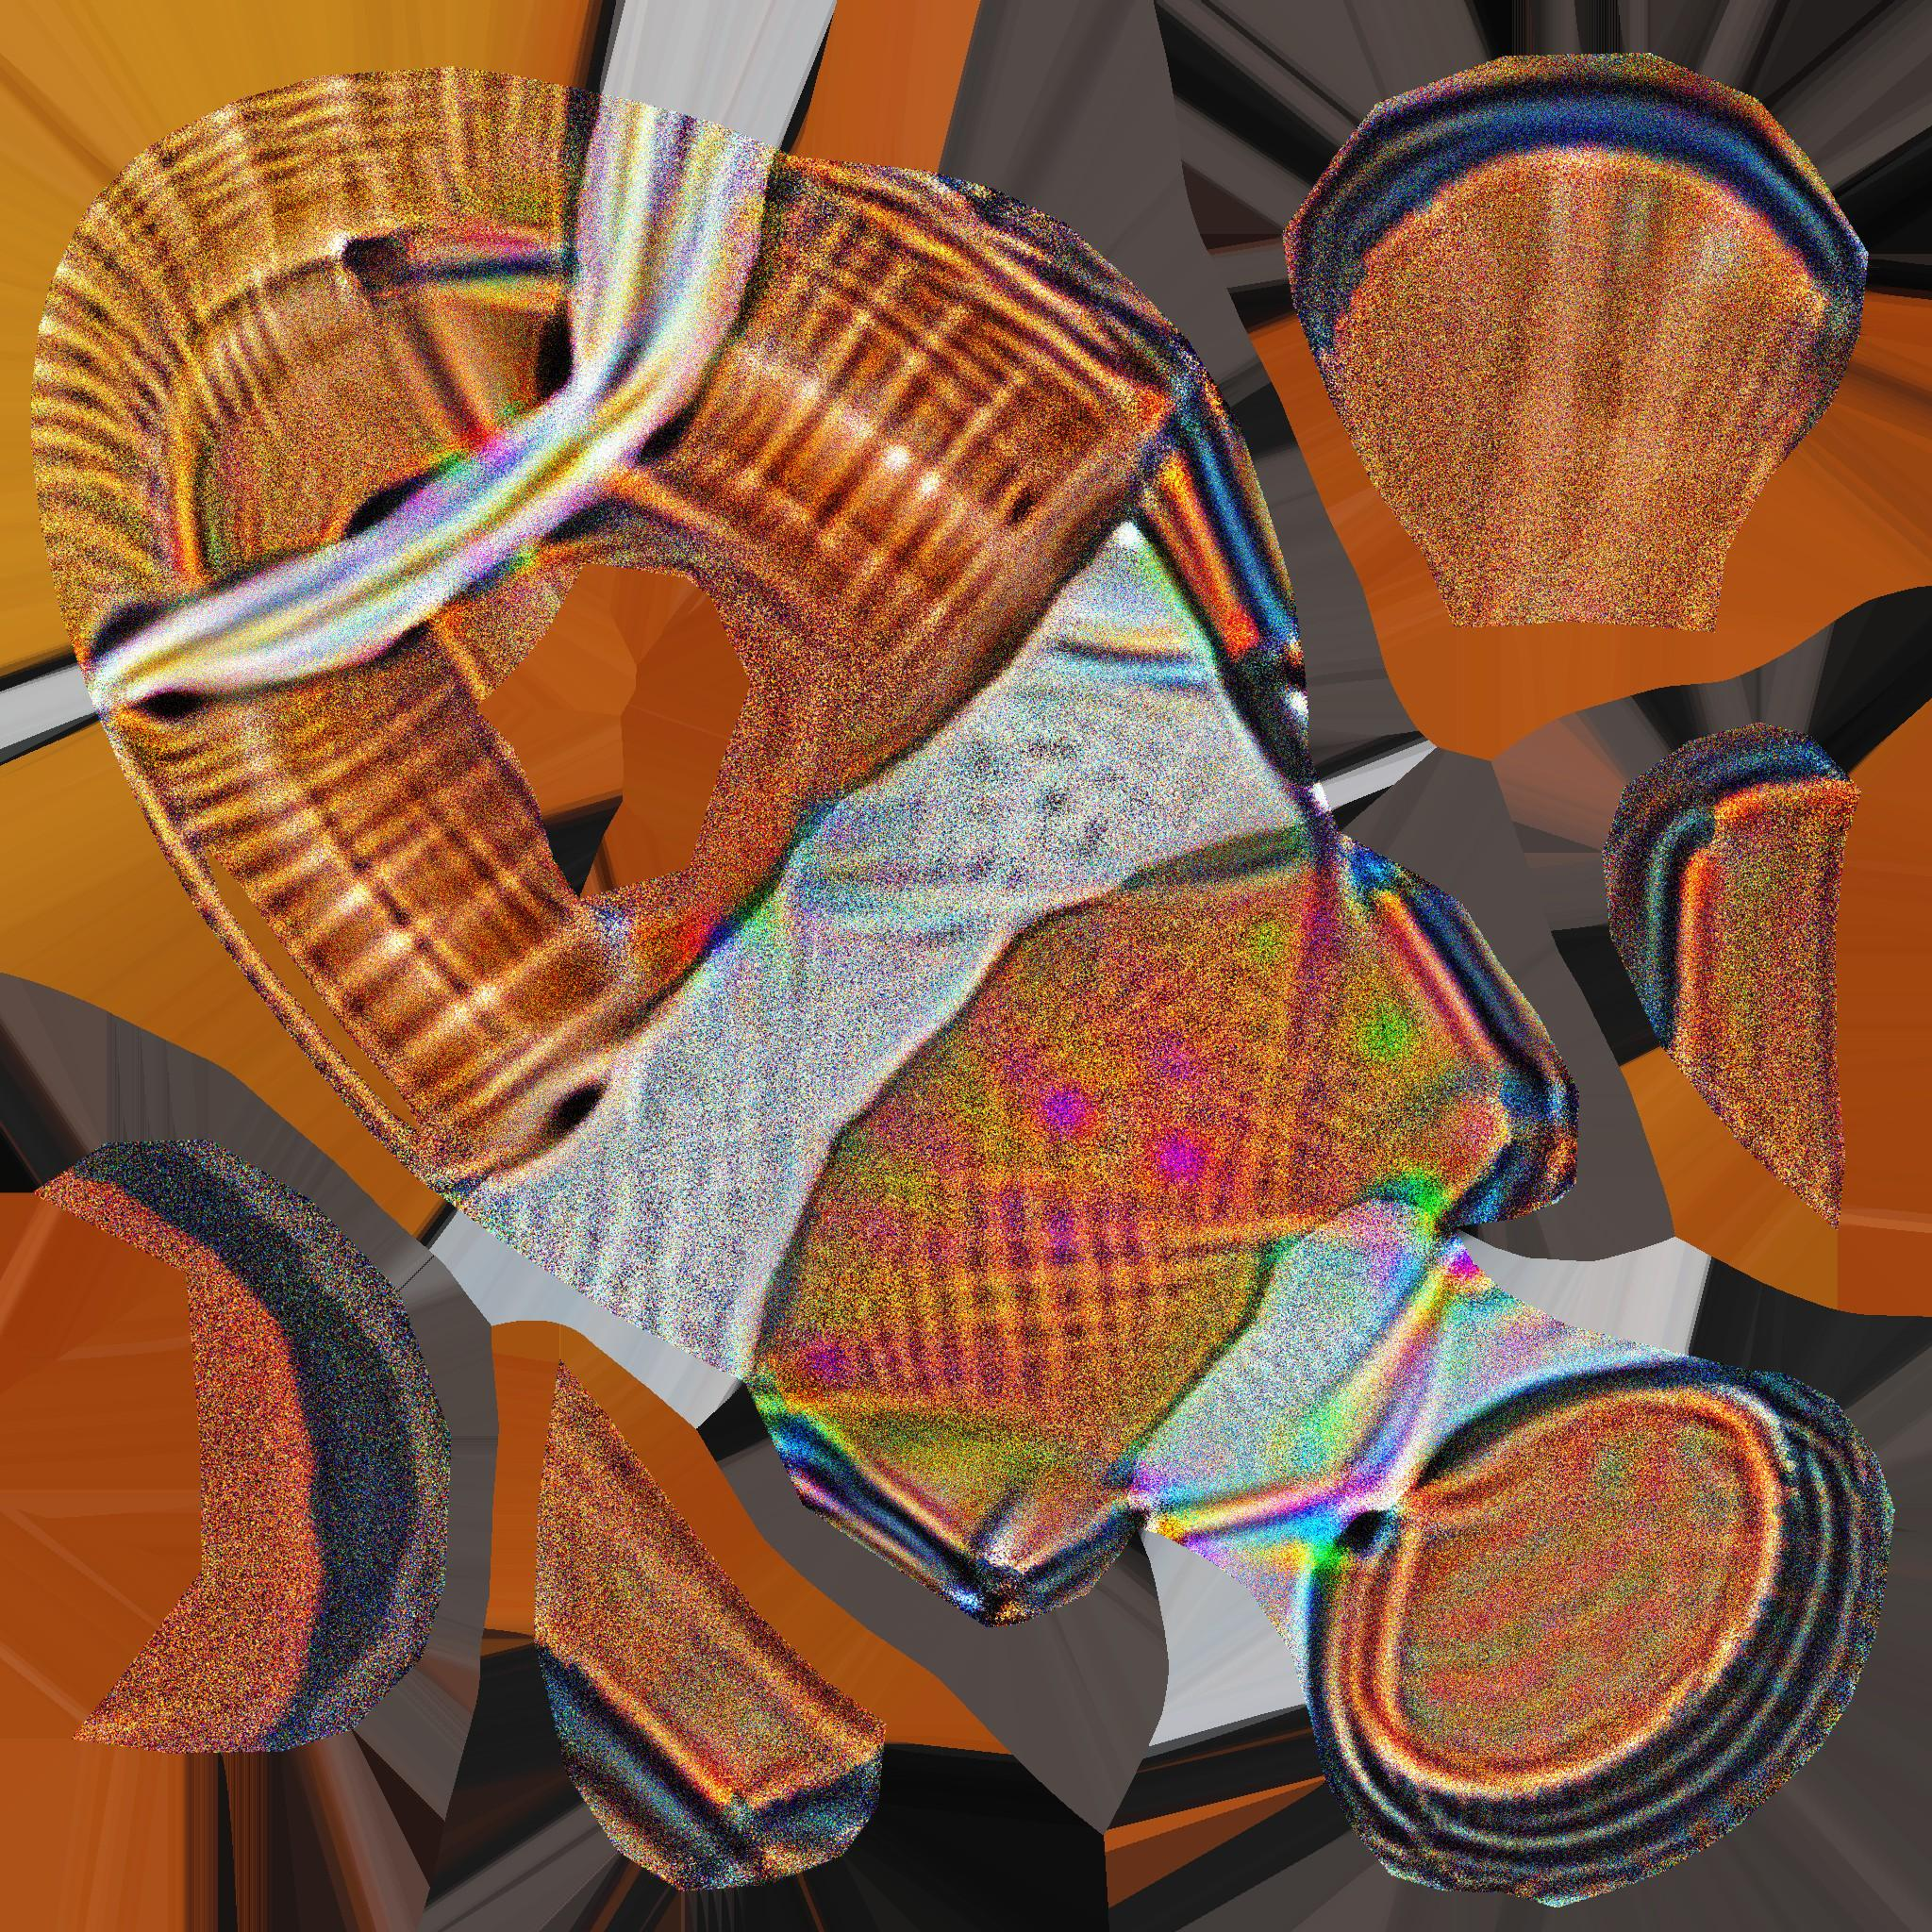
\includegraphics[width=0.6\textwidth]{graphics/clownfish_790_adv_9999.jpg}
    \caption{Adversarial texture for the clownfish model and target label shopping basket. Its TFR is 71\%.}
    \label{fig:clownfish_noisy_texture}
\end{figure}

\begin{figure}[H]
    \centering
    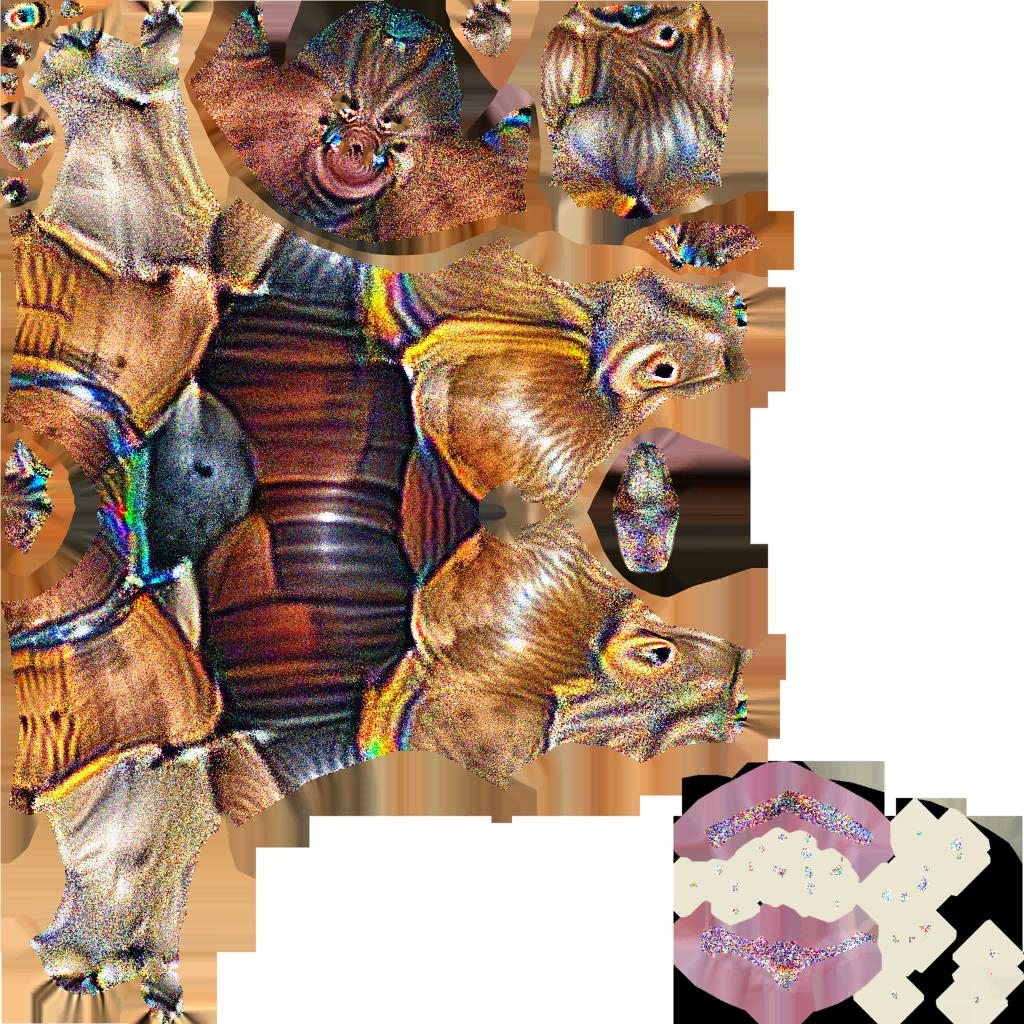
\includegraphics[width=0.6\textwidth]{graphics/german_shepherd_427_adv_9999.jpg}
    \caption{Adversarial texture for the german shepherd model and target label barrel. Its TFR is 76\%.}
    \label{fig:dog_noisy_texture}
\end{figure}

\subsubsection{Reusing renders between optimisation steps}

Some ad-hoc experiments done with the barrel model, before the experiment in subsection \ref{subsec:eot_experiment_design}, show that re-using 80\% of renders versus re-using none has little effect in terms of the TFR of adversarial texture. However, it greatly speeds up the EOT algorithm, as it can do the same number of optimisation steps in less than half the time. This shows that one of the most computationally intensive parts of EOT is the computation of UV maps and using the latter to render 2D images of the objects, as Athalye \textit{et al.} \cite{athalye} also suggested.

\subsubsection{Semantic adversarial perturbations}

A key characteristic of the adversarial noise made for textures of 3D objects by EOT is that they show semantically meaningful patterns related to the target class. A different experiment from the one described in subsection \ref{subsec:eot_experiment_design}, on the crocodile 3D model and target label compass, resulted in the texture in figure \ref{fig:crocodile_compass}. EOT added noise on the belly and back of the crocodile with an oval or circular shape, the same shape a compass has. Similarly, you can see in figure \ref{fig:running_shoe_strawberry} that EOT added green spots, reminiscent of the green seeds on a strawberry, for an adversarial texture of the running shoe model for target label strawberry.

\begin{figure}[H]
    \centering
    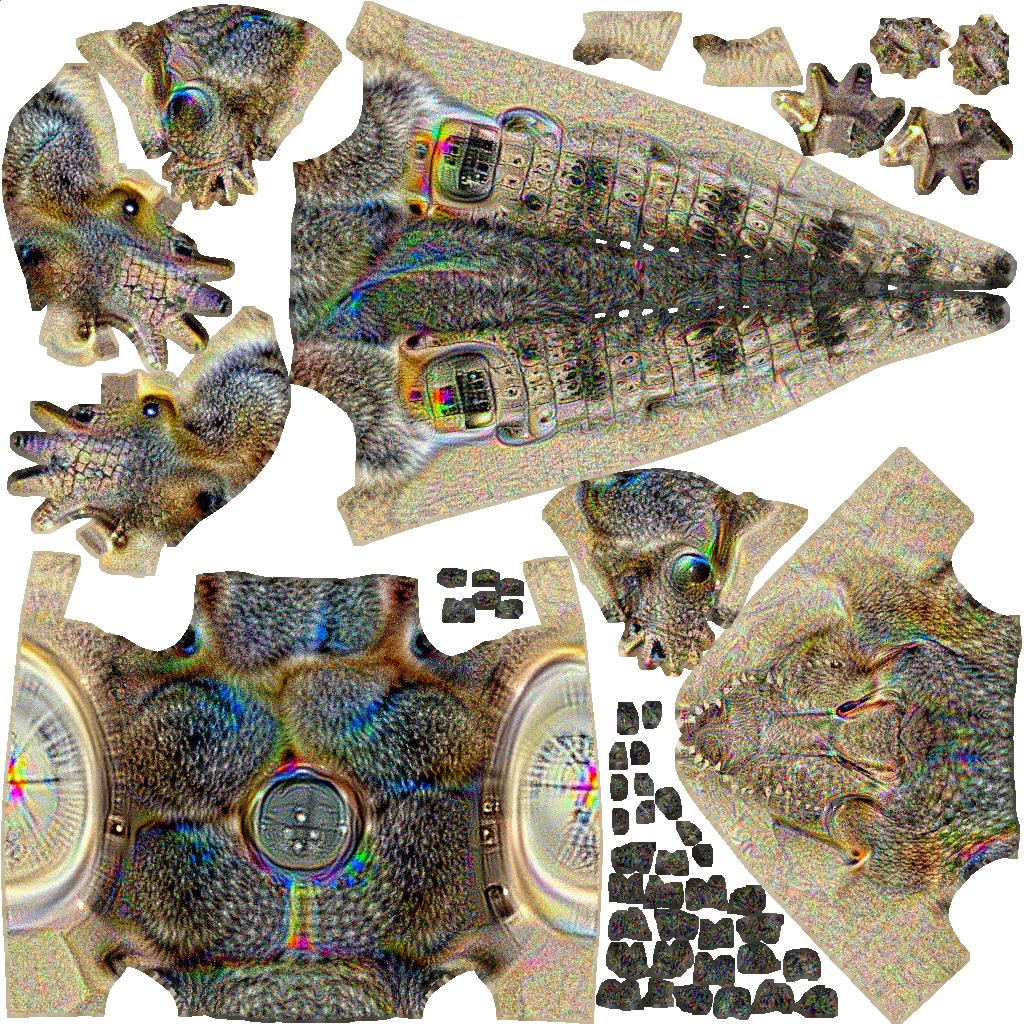
\includegraphics[width=0.55\textwidth]{graphics/crocodile compass.jpg}
    \caption{Adversarial texture for the crocodile model and target label compass. It has a TFR of 60\%.}
    \label{fig:crocodile_compass}
\end{figure}

\begin{figure}[H]
    \centering
    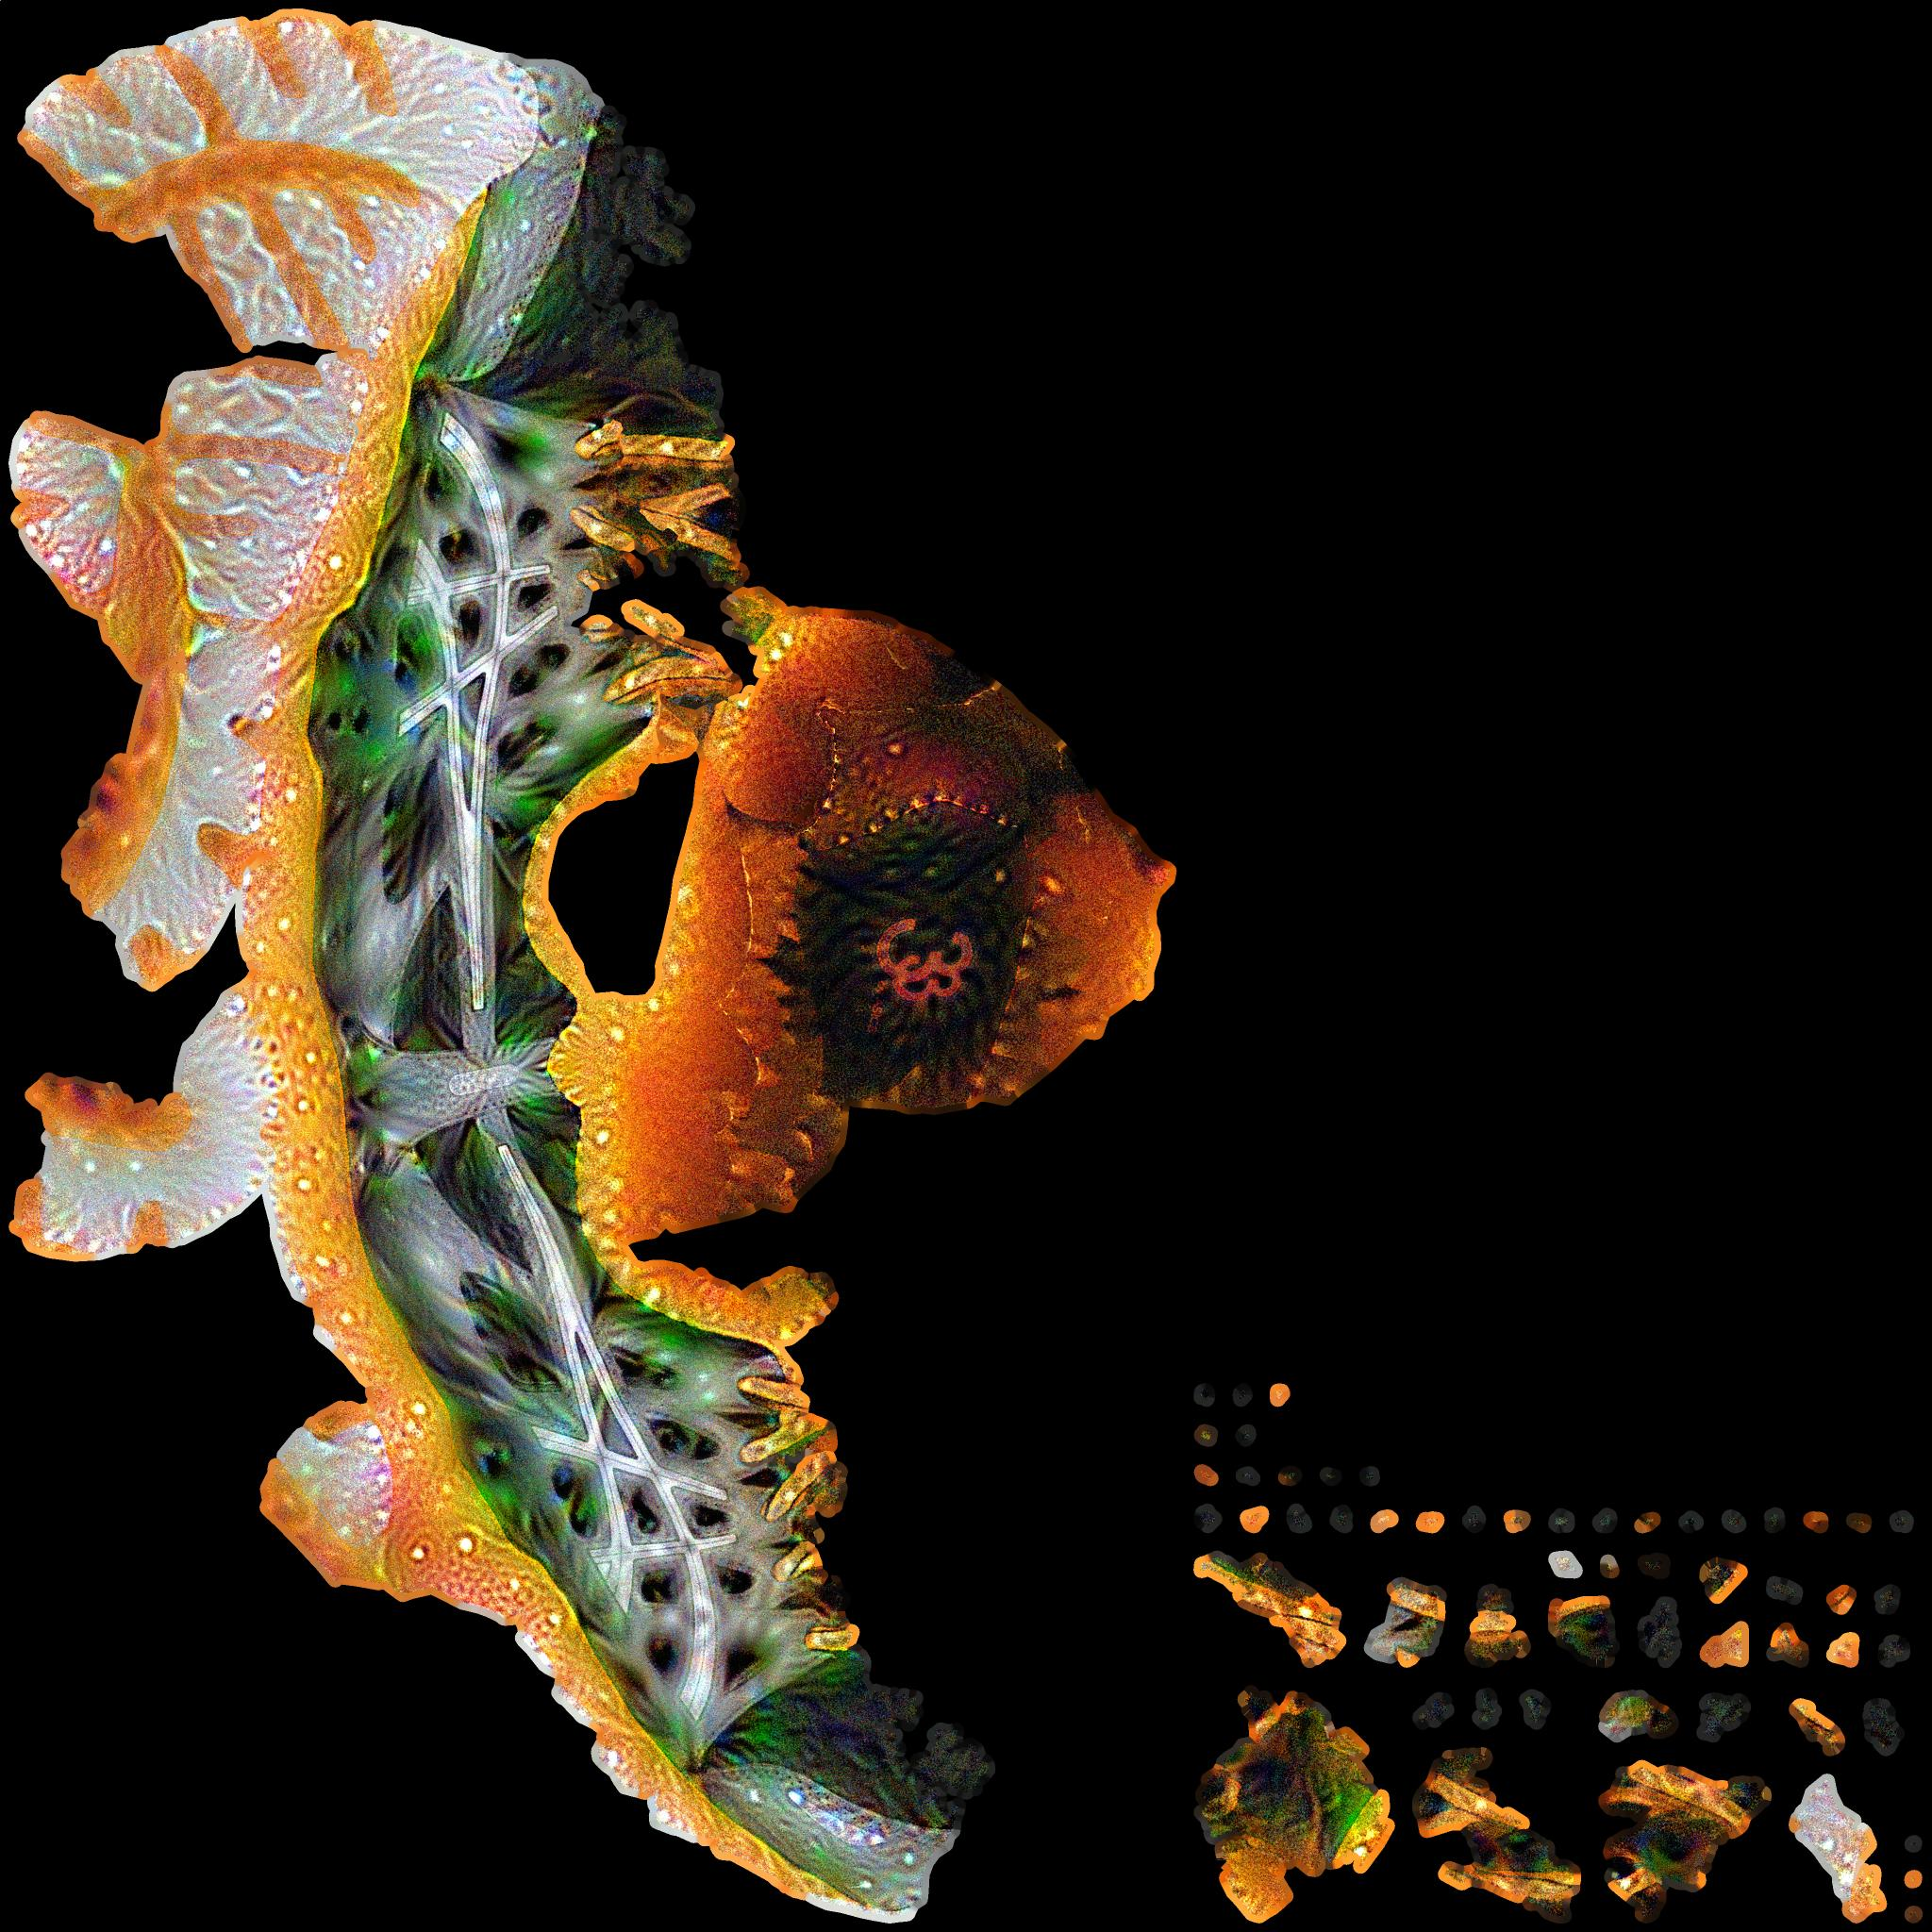
\includegraphics[width=0.55\textwidth]{graphics/running shoe strawberry.jpg}
    \caption{Adversarial texture for the running shoe model and target label compass. It has a TFR of over 80\%.}
    \label{fig:running_shoe_strawberry}
\end{figure}

Another example is in figure \ref{fig:running_shoe_rifle}, where the adversarial texture for the running shoe and label rifle exhibits metallic patterns in the shape of a gun barrel. Given that these three adversarial textures have a significant TFR, they highlight features that the InceptionV3 victim model learned for recognising a compass, strawberry and rifle, respectively. Therefore, EOT can be used to study the explainability of a neural network, as it highlights class features that make the neural network classify a completely different object as that class.

\begin{figure}[H]
    \centering
    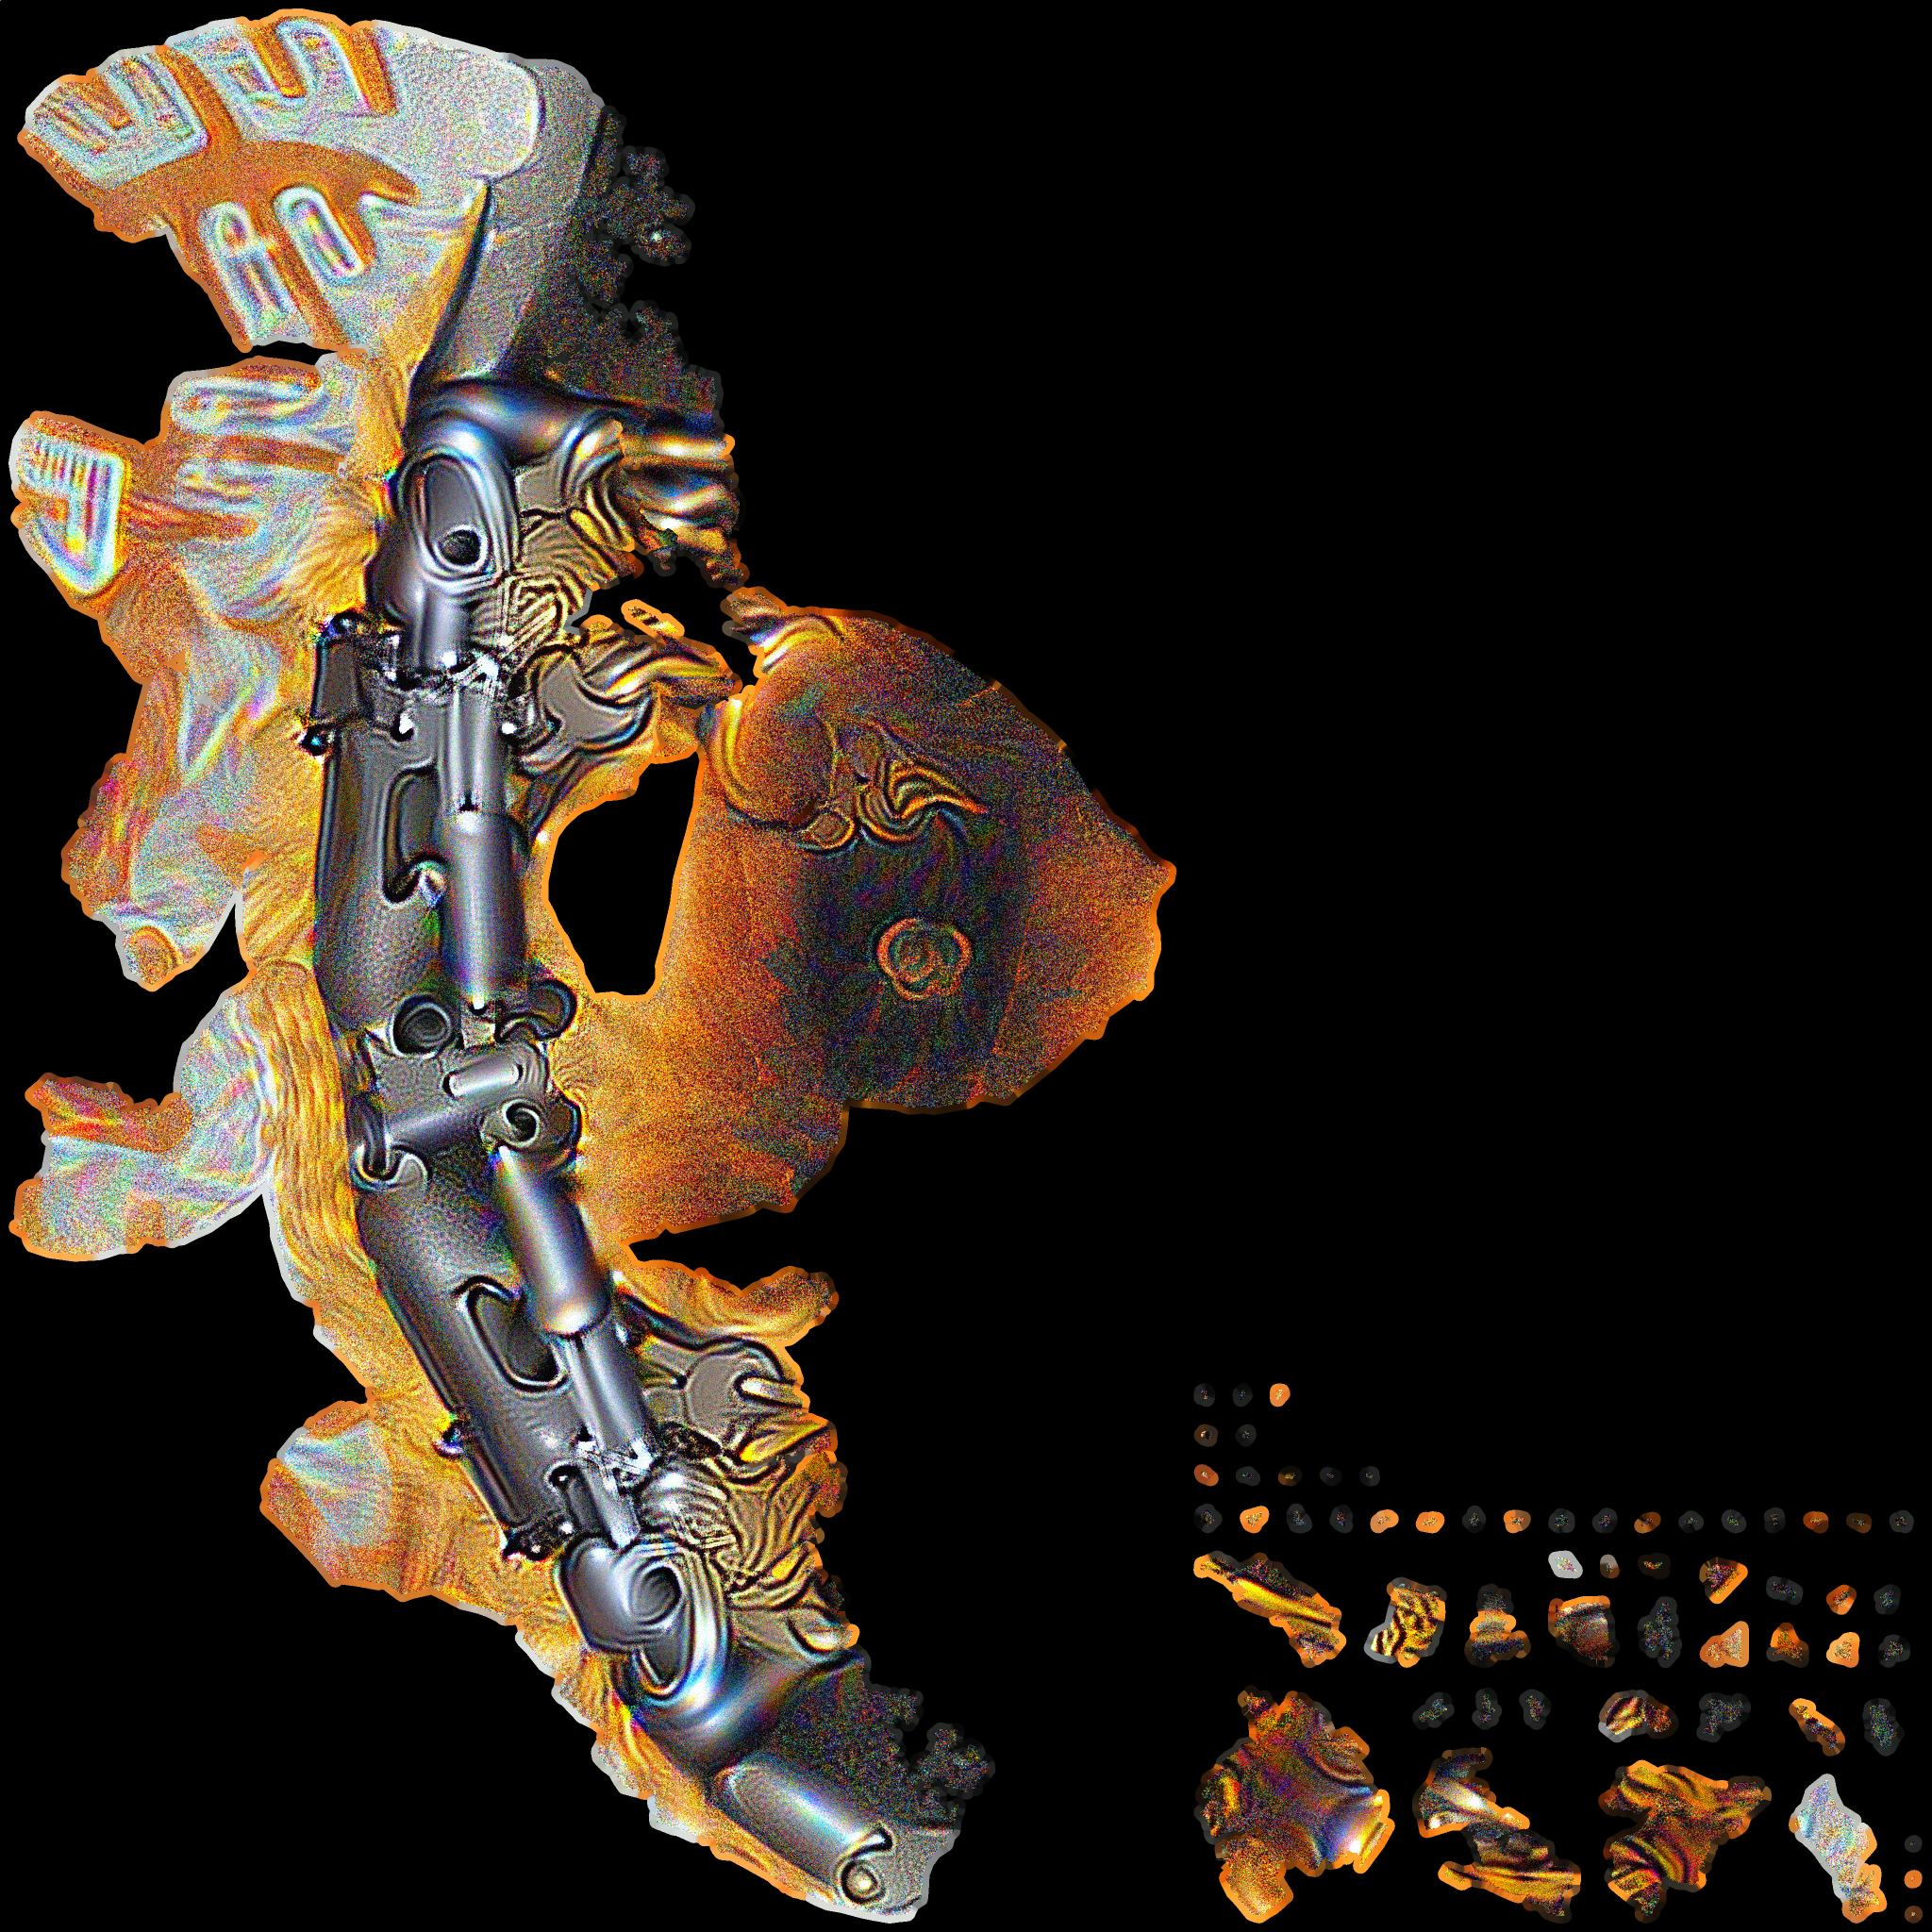
\includegraphics[width=0.55\textwidth]{graphics/running shoe rifle.jpg}
    \caption{Adversarial texture for the running shoe model and target label rifle. It has a TFR of 45-50\%.}
    \label{fig:running_shoe_rifle}
\end{figure}

\section{G-EOT}

\subsection{Experiment Design}

The purpose of this experiment is to see if G-EOT able to learn to create adversarial noise for textures. The model is evaluated by training it using the process described in subsection \ref{subsec:training}. Firstly, the simulator is warmed-up for 2000 training steps. Following that, the G-EOT model is trained for 40000 steps, where each one consists of one simulator training step and one generator training step. This number was chosen because training the model made by Zheng \textit{et al.} \cite{zheng_black_box_GAN} took around 30000 steps to achieve the results seen in their paper, and G-EOT has a harder generation task. Every 500 training steps, the generator is evaluated on 200 batches of new data samples.

The model is trained on the dataset of 15 3D models presented in section \ref{sec:dataset}. At each training step, the batch is made up of randomly picked models out of this dataset. For each model in the batch, random parameters are sampled for translation, rotation and distance from the camera, and a UV map is computed based on those. Moreover, a random target label is sampled from a uniform distribution. It can be any of the 1000 Imagenet labels, except the correct labels for that model. Therefore, each element in the batch is a randomly picked model, with a UV map for a random pose and a random target label. In this experiment, the batch size is 5, as that is the maximum that will fit with 8 GB of VRAM.

The bounds for the uniform distributions used for sampling the camera distance, X/Y translation, additive and multiplicative lighting, and the standard deviation of the gaussian noise, are the same as those used for the EOT experiment in subsection \ref{subsec:eot_experiment_design}. This experiment does not scale the texture before rendering in order to simulate 3D printer errors, as the adversarial 3D models will not be physically printed.

The number of experts in the decoder is 50, as having one expert for each of the 1000 Imagenet labels would be too much, different combinations of expert outputs can used for each target label. The simulator uses an Adam optimiser with an exponentially decaying learning rate. The initial learning rate is 0.001, with a decay rate of 0.98, and it decays after every 300 steps. The generator uses a constant learning rate of 0.004. The reason is that the random renders can lead to strong fluctuations in the loss function value, as you have seen in subsection \ref{subsec:eot_experiment_results}, and a large constant learning rate mitigated that and improved performance for EOT experiment in \ref{subsec:eot_experiment_results}. The gradients of the generator loss function are clipped to a range between -1 and 1, as Zheng \textit{et al.} \cite{zheng_black_box_GAN} also did.

The noise produced by the G-EOT generator has individual values for each pixel between -25 and 25, to be applied to images with pixel values between 0 and 255. The reason behind this limitation is when training starts, the randomly initialised weights are very small, and therefore the values generated noise tends towards 0. When they are scaled to values between -1 and 1, these values are mostly -1. When added to a texture with pixel values between 0 and 1, this resulted in a completely black image. The simulator would not provide a useful gradient to the generator when given a black image, and therefore I introduced this limitation to avoid this. Further work should look into initialisation techniques to avoid this issue.

The weight $\beta$ from equation \ref{eq:g-eot-l2-loss} on page \pageref{eq:g-eot-l2-loss} has a value of 0.001, chosen to relax the constraint on the size of the adversarial noise and make the learning task for the generator easier. Finally, the weight for L2 regularisation of the weights of the simulator and generator is $0.5 * 10^{-4}$, and the simulator and generator's weights are initialised with Orthogonal Initialisation, which was used in BigGAN \cite{big_gan}.

\subsection{Experiment Results}
    \label{sec:experiment_design}
    
You can see a history of the loss of the model in figure \ref{fig:g_eot_loss_history}. The orange plot denotes the value of the first term of equation \ref{eq:generator_loss} on page \pageref{eq:generator_loss}, which measures how close is the generator to fooling the simulator. The green plot denotes the value of the term seen in \ref{eq:g-eot-l2-loss} on page \pageref{eq:g-eot-l2-loss}. The red line represents the average generator loss at each evaluation step, which is done once every 500 training steps, as mentioned in the previous subsection. Moreover, this test loss is calculated by using the victim model rather than the simulator, as fooling the victim model is the intended objective.
    
\begin{figure}[H]
    \centering
    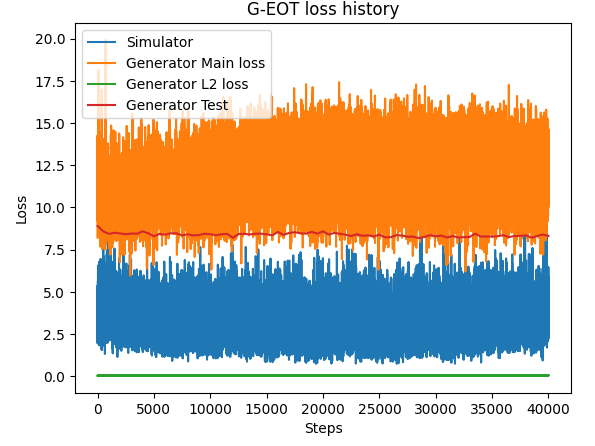
\includegraphics[width=1\textwidth]{graphics/g-eot-loss-history.PNG}
    \caption{Loss history during training for the G-EOT model.}
    \label{fig:g_eot_loss_history}
\end{figure}

The figure shows that the gradient for the generator fluctuates wildly between training steps. Moreover, despite a small decrease in the generator main loss and the generator test loss at the very beginning, they do not decrease further during training. Therefore, the generator failed to learn almost anything, having a TFR of almost 0\% for new random renders sampled during evaluation steps.
    
\subsection{Discussion}

 	%\chapter{Typesetting your thesis}
	\label{chap:typesetting}
	
	This document is intended as both a LaTeX thesis template and as a tutorial on structuring and typesetting your thesis in the LaTeX programming language.
	
	The following are some powerful online resources for learning about LaTeX:
	
	\begin{description}	
			
		\item[$\bullet$ Overleaf Documentation for LaTeX]\hfill
		
		Overleaf \cite{overleafdocs} is an online browser-based LaTeX IDE which stores your document in the cloud and provides live recompilation as you type. The documentation on Overleaf's website has a good knowledge base of examples for how to typeset things cleanly and simply in LaTeX code. 
		
		\noindent See: {\small \url{https://www.overleaf.com/learn}}
		
		\item[$\bullet$ TeX StackExchange, the StackOverflow site dedicated to TeX questions]\hfill
		
		TeX StackExchange \cite{texstackexchange} is sub-community of the StackOverflow network dedicated to questions about the TeX family of typesetting tools including LaTeX, BibTeX and others. A vast majority of the time it is unlikely that the question or issue you are facing is one that has not been encountered before, and this site more than likely to be able to point you in the correct direction. 
		
		\noindent See: {\small \url{https://tex.stackexchange.com}}
		
	\end{description}
	
	\newpage 
		
	\section{Referencing items within this document}
		In section \ref{sec:resources_bibtex} we saw examples of how to typeset citations for resources we had stored in an external BibTeX file. However, often we would like to accurately refer to the location of a resource or region of text stored somewhere else within this document\footnote{Like at the beginning of the last sentence when we referred to section \ref{sec:resources_bibtex}.}. To do this we need to annotate our LaTeX code with \lstinline|\label{key}| statements which will take on the numeric (or otherwise formatted) identifier for the current chapter, section, figure, table, equation, ect where they are directly defined. To insert an inline reference to the label you can use the \lstinline|\ref{key}| command which works similarly to the \lstinline|\cite{key}| used for external references. In the event we chose to reorder or add additional content to the document, which would change the section numbering, the document will still compile to a pdf with the correct references inserted for each \lstinline|\ref{key}| command.
		
	\section{Equations}
	\label{sec:typesetting_equations}
	
	Typesetting equations is one of the things that LaTeX does best. It has packages for different fonts and symbols for many different mathematical notations. However, to person learning how to typeset in LaTeX for the first time it can be a daunting and unwieldy user experience. Almost all LaTeX packages have documentation available in pdf format online, and documentation for packages specifically relating to fonts and symbols usually have tables enumerating the names and codes for all of the fonts symbols, organized by intended usage. 
	
	\subsection{Inline equations}
	
	Small equations like $x = 0$ can be written directly within the text by using LaTeX's maths mode shorthand controlled by dollar signs \lstinline|$ math mode $|. As long as it is not becoming cumbersome to the reader, equations such as $\mathbb{P}({A} \cap {B}) = \mathbb{P}({B} \cap {A})$ are quite neatly displayed in this fashion. 
	
	\newpage 
	
	\subsection{Block equations}
	
		For long equations it is best to provide a break in the main text of the document and format the equation using a \lstinline|\begin{equation}...\end{equation}| environment. 
		
		\begin{equation} \label{eq:veclen}
			\left\lvert a \right\rvert = \left\lvert \left[\begin{array}{c} a_0\\ a_1\\ \vdots\\ a_n\end{array}\right] \right\rvert = \sqrt{a_0^2 + a_1^2 + \hdots + a_n^2}
		\end{equation}
		
		Equation \ref{eq:veclen} demonstrates formatting a larger equation and uses an \lstinline|\begin{array}...\end{array}| environment to structure a column vector of sub-equations. Block equations should be located at a relevant point directly as they are being referred to in the text. When referred to from other locations in the document you should use the \lstinline|\ref{key}| command to insert the correct equation number.
		
		\subsubsection{Aligning multi-line block equations}
		
			When equations become even larger they may need cross over multiple new lines. When this happens it is desirable to align relevant parts of the equation on each line to one another for aesthetic reasons and to help imply structure to the reader. 
		
			\begin{equation} \label{eq:rendering_equation}
				\begin{split}
					\mathcal{L}_o\left(x, \omega_o, \lambda, t\right) &= \mathcal{L}_e\left(x, \omega_o, \lambda, t\right)\\
					&+ \int_\Omega f\left(x, \omega_i, \omega_o, \lambda, t\right) \mathcal{L}_i\left(x, \omega_i, \lambda, t\right) \left(\omega_i \bullet n\right) d\omega_i\\
					&\text{where} \quad \mathcal{L}_i\left(x, \omega_i, \lambda, t\right) = \mathcal{L}_o\left(x^\prime, -\omega_i, \lambda, t\right)\\
				\end{split}
			\end{equation}
			
			Equation \ref{eq:rendering_equation}, known as Kajiya's Rendering Equation \cite{kaj86} demonstrates the use of the \lstinline|\begin{split}...\end{split}| environment which uses a single un-escaped \& symbol placed on each line of the equations LaTeX code to indicate where each line should be co-aligned. In this example the \&'s were placed on the =, +, and w (in where) characters.
			
	\subsection{A masochistic approach to learning to typeset mathematics in LaTeX}
	
		% [H] means put the figure HERE, directly when you input this code.
\begin{figure}[H]
	\centering
	
% Note we use the frame option to make latex put a 1 pixel black border around the image.
% This is useful when the image has a white  or transparent background and will be displayed on white.
	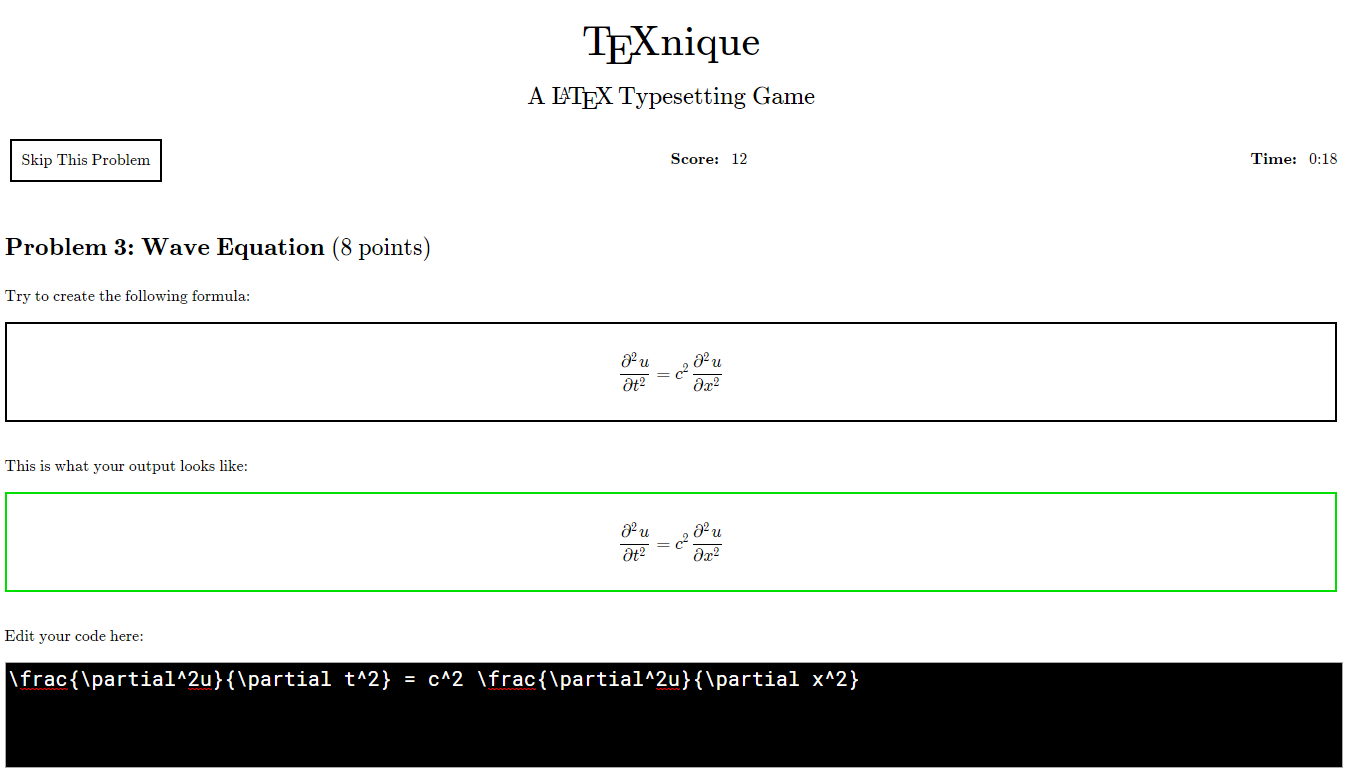
\includegraphics[width=1.0\linewidth,frame=]{./graphics/texnique.png}

% Caption is defined with a short and long version. The short version is shown in the 
% List of Figures section, and the long version is used directly with the figure. 			
	\caption[A screenshot of TeXnique, a game about typesetting equations.]{TeXnique, a game about typesetting equations \cite{texnique}. (Top) The game presents you with a rendered equation, (Bottom) the task is to enter LaTeX code that produces the same rendered equation. The green border on the lower rendering indicates it is a valid solution.}
	
% For figures label should be defined after the caption to ensure proper figure numbering.
	\label{fig:texnique}
\end{figure}
		
		TeXnique \cite{texnique} is web-browser based game for practising how to typeset equations in LaTeX. The game will present you with a rendered equation and your task is to type LaTeX code into the box below it such that your code produces the same (or closely matching / pixel equivalent) rendered equation. Figure \ref{fig:texnique} shows the game during play, the bottom rendered equation is bordered in green to indicate it is a valid match with the target. 

		% An example of how to center a passage of text, control local fontsize, 
		% and create a properly formatted and clickable URL.
		\begin{center}
		{\small \url{https://texnique.xyz}}
		\end{center}
		
		This is one of the more painful parts of typesetting a document, so it really takes a special kind of sadism to come up with such a game. Least to say, graduate students and researchers can be an odd bunch, and when we found this it was surprisingly addictive to compete over. 
		
		
		
	\section{Figures}
	\label{sec:typesetting_figures}
	
	In this template figures are numbered starting with the current chapter number followed by a figure number that resets to 1 each new chapter. As you can see below, the first figure is labelled Figure \ref{fig:dragon} because we are in Chapter \ref{chap:typesetting}.
	
	Figures in LaTeX are defined using a \lstinline|\begin{figure}...\end{figure}| environment and often immediately begin rendering in centre aligned mode by calling \lstinline|\centering|. Listing \ref{lst:latex_figure} below shows the LaTeX code used to typeset figure \ref{fig:dragon}. Figures \ref{fig:example_2x1} and \ref{fig:example_2x2} are defined similarly and make additional use of the \lstinline|\subfloat| command to position multiple images within a single figure environment, each with their own automatically incremented labels and individual captions.

	\lstinputlisting[label={lst:latex_figure}, caption={An example LaTeX excerpt demonstrating how to typeset figure \ref{fig:dragon} with a simple caption.}]{./listings/example_figure.tex}

	\subsection{Consistent presentation throughout the document}
		Figures work best in a document when you use a consistent style for formatting and captioning them and make sure that figures always actively support the content of the main text. 
	
	\subsection{Justified use of space in the document}
		All figures must be referred to directly in the main text of the document and discussed with meaningful and in depth critical analysis. If you don't need to use the figure to leverage and support your discussion then it is just taking up space and padding out the document. For example, you can use a command like \lstinline|\ref{fig:dragon}| to automatically get the figure number for Figure \ref{fig:dragon}. 	
		
		% [H] means put the figure HERE, directly when you input this code.
\begin{figure}[H]
	\centering

% We set the width of the figure based on the width of one line of text on the page. 
% The value can be tuned to any value in [0.0, 1.0] to scale the image while maintaining its aspect ratio.
	\includegraphics[width=1.0\linewidth]{./graphics/dragon.png}
	
% Caption is defined with a short and long version. The short version is shown in the 
% List of Figures section, and the long version is used directly with the figure. 		
	\caption[An image of many glass dragons being used to demonstrate typesetting a figure.]{A good caption should be sufficient enough to put the figure in context even if the reader has randomly flicked to the current page and looked only at the figure in isolation. All figures should also be referred to directly within the main text of your document. You can use the LaTeX \textbf{$\backslash$ref\{key\}} command to insert the correct figure number when you refer to it in the main text. By the very logic of this caption, this is a very poor caption because we still don't know why on earth is there an picture of glass dragons here. Image of glass dragons rendered using Path Tracing \cite{whittle15_dragons}.}
	
% For figures label should be defined after the caption to ensure proper figure numbering.
	\label{fig:dragon}
	
\end{figure}
		
	\subsection{Placement that supports and enhances the flow of the document}
		All figures shown in your document should be displayed in relevant locations, ideally just after that have been alluded to in the main text. Although there are many times where it is best to force a figure to the top or bottom of a nearby page.
	
	\subsection{Avoid directly importing other peoples images}
		You should avoid using other peoples figures whenever possible, and instead create your own figures for visualizing the specific methods and data you are working with in a way directly relevant to your project. 
	
	\subsection{Format sub-figures in LaTeX, not in the image itself}
		Construct sub-figures from multiple image files in LaTeX not in the image file itself. This allows you to tweak the positioning and layout without having to modify the images. It also allows for automatic formatting and numbering of captions and sub-captions. Figures \ref{fig:example_2x1} and \ref{fig:example_2x2} show examples of side-by-side and quad layouts respectively.
		
		% [H] means put the figure HERE, directly when you input this code.
\begin{figure}[H]
	\centering
	
% We use a figure width of 48.5% of the width of one line of text on 
% the page so there is some space between the images.
	\subfloat[Left image sub-caption.]{
		\includegraphics[width=0.485\linewidth]{./graphics/dragon.png}\label{fig:example_2x1_a}
	}~ % Use a tilde to add spacing for sub-figures that are displayed next to one another horizontally.
	\subfloat[Right image sub-caption.]{
		\includegraphics[width=0.485\linewidth]{./graphics/dragon.png}\label{fig:example_2x1_b}
	}\\ % New line before caption.

% Caption is defined with a short and long version. The short version is shown in the 
% List of Figures section, and the long version is used directly with the figure. 	
	\caption[A demonstration of a 2x1 sub-figure layout.]{Construct sub-figures from multiple image files in LaTeX not in the image file itself. This allows you to tweak the positioning and layout without having to modify the images. It also allows for automatic formatting and numbering of captions and sub-captions. Image of glass dragons rendered using Path Tracing \cite{whittle15_dragons}.}
	
% For figures label should be defined after the caption to ensure proper figure numbering.
	\label{fig:example_2x1}
	
\end{figure}
		
		% [H] means put the figure HERE, directly when you input this code.
\begin{figure}[H]
	\centering
	
% We use a figure width of 48.5% of the width of one line of text on 
% the page so there is some space between the images.
	\subfloat[Top-Left image sub-caption.]{
		\includegraphics[width=0.485\linewidth]{./graphics/dragon.png}\label{fig:example_2x2_a}
	}~ % Use a tilde to add spacing for sub-figures that are displayed next to one another horizontally.
	\subfloat[Top-Right image sub-caption.]{
		\includegraphics[width=0.485\linewidth]{./graphics/dragon.png}\label{fig:example_2x2_b}
	}\\ % New line before caption.
	\subfloat[Bottom-Left image sub-caption.]{
		\includegraphics[width=0.485\linewidth]{./graphics/dragon.png}\label{fig:example_2x2_c}
	}~ % Use a tilde to add spacing for sub-figures that are displayed next to one another horizontally.
	\subfloat[Bottom-Right image sub-caption.]{
		\includegraphics[width=0.485\linewidth]{./graphics/dragon.png}\label{fig:example_2x2_d}
	}\\ % New line before caption.
		
% Caption is defined with a short and long version. The short version is shown in the 
% List of Figures section, and the long version is used directly with the figure. 	
	\caption[A demonstration of a 2x2 sub-figure layout.]{A demonstration of a 2x2 sub-figure layout. Between A-B and C-D we use tilde symbols and between B-C we use a new line. Image of glass dragons rendered using Path Tracing \cite{whittle15_dragons}.}
	
% For figures label should be defined after the caption to ensure proper figure numbering.
	\label{fig:example_2x2}
	
\end{figure}
	
	\subsection{Robust captions that can stand in isolation}
		Figures need to be captioned such that they can be viewed in isolation and still be meaningful to the viewer. There will likely be some duplication of information that is written in the main text, but this is intended. 
	
	\subsection{Proper attribution and citation of images}
		\label{sec:typesetting_figures_citation}
		
		If an image does not belong to you it \textbf{must} be cited directly in the figure caption. \textbf{It is not correct to put a URL in the figure caption directly.} A URL in isolation is not an accurate or reliable way of directing a future reader to the exact content you are referencing. Instead make a new entry in your \lstinline|citations.bib| file and then reference that citation in the caption using the \lstinline|\cite{key}| command. Figures \ref{fig:dragon}, \ref{fig:example_2x1}, and \ref{fig:example_2x2} each include a statement in the caption stating ``Image of glass dragons rendered using Path Tracing \cite{whittle15_dragons}.''. When adding the BibTeX entry, try to find the proper information about the original author and source document to strengthen the citation in case the URL changes. 
	
	\section{Code Listings}
	\label{sec:typesetting_listings}
	
	Code listings should be formatted in the same style as figures and inline equations. It is important to use a monospace font so that characters line up vertically. Syntax highlighting is also extremely important for effectively displaying complicated code segments. To format inline code listings you can use the \lstinline[mathescape]|\lstinline$|$the_code$|$| command\footnote{So meta.}.
	
	% Longform Code listings should live in a code file, not embedded directly into your LaTeX code!
	\lstinputlisting[language={c}, label={lst:c_hello_world}, caption={An implementation of an important algorithm from our work.}]{./listings/hello_world.c}
	
	In LaTeX the ``Listings'' package can be used to properly format code and provide basic syntax highlighting, line numbering, and captioning of embedded code excerpts. Listing \ref{lst:listings} shows examples of how to properly format code using the listings package. 
	
	\newpage
	
	% Longform Code listings should live in a code file, not embedded directly into your LaTeX code!
	\lstinputlisting[label={lst:listings}, caption={Examples of methods for typesetting code listings within a LaTeX document.}]{./listings/listings.tex}
	
	\section{Tables}
	\label{sec:typesetting_tables}
	
	Tables are also quite predictably captioned and formatted the same way. It is important to decide on a style for how you will organize your data and apply that style consistently for all of your tables. Table \ref{tbl:example_table} shows one possible way of styling your data but is by no means the only way of doing so neatly. Consistency is the key. 
	
	% It's often a good idea to generate the LaTeX code for tables (python script or similar) so that if you rerun your code you don't have to typeset your results again by hand!
\begin{table}[H]
	\centering
	\scriptsize
	\caption[A demonstration of a table typeset in LaTeX.]{An example of a table formatted with caption.}
	
	% Tune the following two values that are being multiplied by the variable \textwidth
	% to control how large the scale of the table is, and how much is is squashed back 
	% to the final size.	
	\resizebox{0.8\textwidth}{!}{
		\begin{tabularx}{0.46\textwidth}{c|c|c|c|c|c}
			\toprule
			Some & Relevant & Fields & From & Your & Data\\
			\midrule
			0 & 0 & 0 & 0 & 0 & 0\\
			1 & 1 & 1 & 1 & 1 & 1\\
			2 & 2 & 2 & 2 & 2 & 2\\
			\bottomrule
		\end{tabularx}
		\label{tbl:example_table}
	}
\end{table}




	

 	\chapter{Conclusions and Future Work}
\label{chap:conclusion}

In this document we have demonstrated the use of a LaTeX thesis template which can produce a professional looking academic document. 

\section{Contributions} 
\label{sec:conclusion_contributions}

The main contributions of this work can be summarized as follows:
\begin{description}	

	\item[$\bullet$ A LaTeX thesis template]\hfill
	
	Modify this document by adding additional top level content chapters. These descriptions should take a more retrospective tone as you include summary of performance or viability. 
	
	
	\item[$\bullet$ A typesetting guide of useful primitive elements]\hfill
	
	Use the building blocks within this template to typeset each part of your document. Aim to use simple and reusable elements to keep your document neat and consistently styled throughout.
	
	\item[$\bullet$ A review of how to find and cite external resources]\hfill
		
	We review techniques and resources for finding and properly citing resources from the prior academic literature and from online resources. 
	
\end{description}

\section{Future Work}
\label{sec:conclusion_future_work}

	
% Formatting citations properly when they are rendering incorrectly in your PDF can be fiddly,
% espectially when punctuation and international characters are involed. Sometimes multiple re-compilations
% are needed in addition to clearing temporary auxiliary files to see your changes in your document.
% Insert the bibliography using citations contained in the file citations.bib
	\bibintoc%
	\bibliography{citations} 
	
% In the appendix you might include a full code listing for an implemented algorithm that you showed a 
% small chunk of in one of your chapters. If you have extra graphs for ablation style experiments you 
% might enumerate them within the appendix and use \label{name} and \ref{name} to automatically insert 
% the correct section locations when you talk about them in your chapters.
% Within appendix.tex you should use chapters as the top level section dividers.
	\appendix
	\addappheadtotoc
	\chapter{Detailed architecture of G-EOT}
    \label{app:detailed_architecture}

\begin{figure}[h]
    \centering
    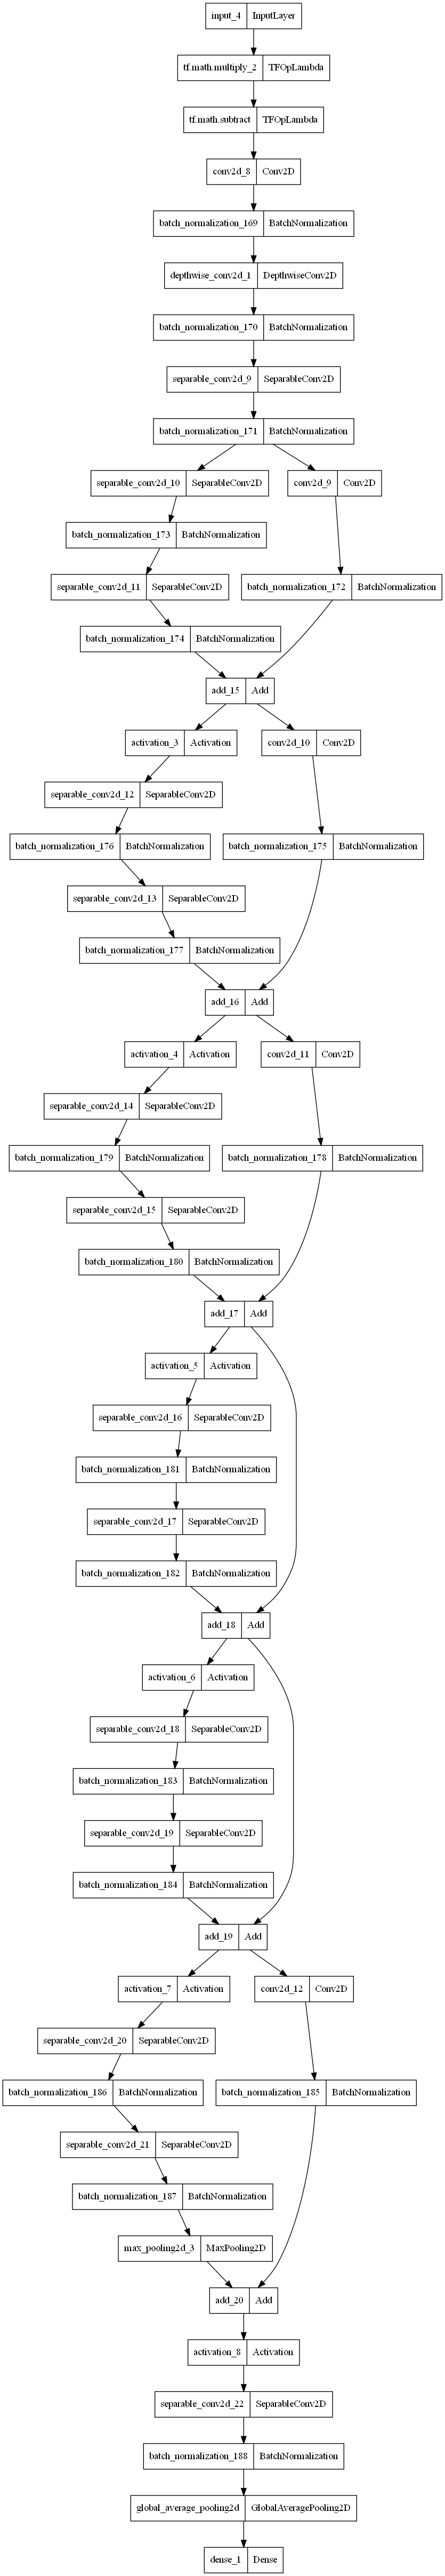
\includegraphics[width=0.24\textwidth]{graphics/detailed_simulator.png}
    \caption{Detailed diagram of the simulator of G-EOT.}
\end{figure}

\chapter{Credits for 3D models}
    \label{app:model_credits}

\begin{table}
\caption{Web links from where each 3D model in the dataset was downloaded.}
\begin{tabular}{|p{1.5cm} | p{12.5cm}|} 
 \hline
 Name & URL \\ [0.5ex] 
 \hline
 \hline
 barrel & https://free3d.com/3d-model/barrel-7685.html \\ 
 \hline
 baseball & https://www.cgtrader.com/free-3d-models/sports/equipment/game-ready-worn-baseball-ball \\ [1ex] 
 \hline
 camaro & https://free3d.com/3d-model/chevrolet-camaro-46813.html \\
 \hline
 crocodile & https://free3d.com/3d-model/crocodile-v1--688517.html \\
 \hline
 clownfish & https://sketchfab.com/3d-models/clownfish-47ba2679d91a4f14b3fc0bf8e3805af5 \\
 \hline
 crocodile & https://free3d.com/3d-model/crocodile-v1--688517.html \\
 \hline
 german shepherd & https://www.cgtrader.com/free-3d-models/animals/other/german-shepherd-dog-203601c4-4783-40e5-ab32-afa14e042dd5 \\
 \hline
 jeep & https://www.cgtrader.com/free-3d-models/car/suv/uaz-3d \\
 \hline
 orange & https://free3d.com/3d-model/-orange--470103.html \\
 \hline
 orca & https://www.cgtrader.com/items/3331128/download-page \\
 \hline
 purse & https://www.cgtrader.com/free-3d-models/household/other/small-bag-wallet \\
 \hline
 rugby ball & https://free3d.com/3d-model/rugby-ball-v1--585369.html \\
 \hline
 running shoe & https://app.gazebosim.org/GoogleResearch/fuel/models/ASICS\_GELBlur33\_20 \_GS\_BlackWhiteSafety\_Orange \\
 \hline
 turtle & https://free3d.com/3d-model/sea-turtle-v1--175922.html \\
 \hline
 taxi & https://free3d.com/3d-model/taxi-v2--375169.html \\
 \hline
 teddy & https://free3d.com/3d-model/teddy-bear-sg-v1--215992.html \\
 \hline
\end{tabular}
\end{table}

\chapter{Adversarial textures created by EOT}
    \label{app:adversarial_textures}

	
\end{document}